% Overleaf: Menu → Compiler → LuaLaTeX に設定してください
% 演讲者视图版本：用 Pympress 打开编译后的 PDF 即可实现演讲者备注
\documentclass[aspectratio=169, 11pt]{beamer}

% ===== Metropolis Theme =====
\usetheme[progressbar=frametitle, numbering=fraction, block=fill]{metropolis}

% ===== Speaker notes on second screen =====
\usepackage{pgfpages}
\setbeameroption{show notes on second screen=right}

% ===== Compress Metropolis spacing =====
\makeatletter
\setlength{\metropolis@frametitle@padding}{1.5ex}
\makeatother
\setlength{\leftmargini}{1em}

% ===== Japanese support =====
\usepackage{luatexja}
\usepackage[haranoaji]{luatexja-preset}

% ===== Packages =====
\usepackage{amsmath, amssymb, mathtools}
\usepackage{physics}
\usepackage{tikz}
\usetikzlibrary{arrows.meta, decorations.pathmorphing, patterns}
\usepackage{xcolor}
\usepackage{booktabs}
\usepackage{graphicx}
\usepackage{siunitx}
\usepackage{appendixnumberbeamer}
% Compress Beamer list spacing (enumitem conflicts with Beamer)
\setbeamertemplate{itemize/enumerate body begin}{\vspace{-0.3em}}
\setbeamertemplate{itemize/enumerate body end}{\vspace{-0.2em}}

% ===== Note page style =====
\setbeamertemplate{note page}{%
  \pagecolor{yellow!5}%
  \vspace{0.5em}
  \begin{minipage}[t]{0.95\textwidth}
    \scriptsize\insertnote
  \end{minipage}
}

% ===== Custom colors =====
\definecolor{accent}{RGB}{230,126,34}
\definecolor{darkblue}{RGB}{23,67,88}
\definecolor{alertred}{RGB}{192,57,43}

\setbeamercolor{frametitle}{bg=darkblue}
\setbeamercolor{progress bar}{fg=accent}
\setbeamercolor{alerted text}{fg=alertred}

% ===== Custom commands =====
\newcommand{\highlight}[1]{\colorbox{yellow!30}{$\displaystyle #1$}}
\newcommand{\importantbox}[1]{%
  \begin{center}
  \fcolorbox{darkblue}{blue!5}{\parbox{0.75\textwidth}{\centering\small #1}}
  \end{center}
}
\newcommand{\teacher}[1]{{\color{darkblue}\textbf{→ #1}}}

% ===== Title =====
\title{物理化学 6}
\subtitle{量子化学の基礎}
\author{大学院入試 備考資料}
\date{}
\institute{化学システム工学専攻}

\begin{document}

\maketitle

\note{
【开场白】\\[4pt]
大家好，今天我们来学习物理化学中的量子化学基础。这是东大化学系统工学专攻修士入试的核心考点之一。\\[4pt]
整个讲座的主线非常清晰：我们要理解"为什么需要量子力学"，然后学会"怎么用薛定谔方程解题"。\\[4pt]
不要被公式吓到，所有推导都有清晰的物理图像支撑。让我们开始吧！
}

% ============================================================
\begin{frame}{この講義の目標}

量子化学は「式が多くて難しそう」と思われがちですが，\\
実は\alert{たった一つの方程式}を解くだけの話です。

\vspace{0.3em}
\importantbox{
  Schrödinger方程式 $\hat{H}\psi = E\psi$ を具体的な$V(x)$のもとで解く → エネルギーと波動関数が分かる
}

\textbf{今日の流れ：}
\begin{enumerate}
  \item なぜ古典力学ではダメなのか？
  \item Schrödinger方程式の導出
  \item 変数分離法 → 井戸型ポテンシャル
  \item 物理的意味と応用（共役ポリエン）
  \item 分子振動（調和振動子・Morse）
  \item 黒体放射の定量（Wien則・Stefan-Boltzmann則）
\end{enumerate}
\end{frame}

\note{
【讲解要点】\\[4pt]
这一页是整个讲座的路线图，先让听众知道今天要干什么。\\[4pt]
\textbf{核心信息：}量子化学看起来公式很多，但本质上就是一件事——给定一个势能函数$V(x)$，代入薛定谔方程，解出能量$E$和波函数$\psi$。\\[4pt]
\textbf{讲解顺序：}\\
1. 先讲"为什么需要量子力学"（黑体辐射、光电效应、德布罗意波）——建立动机\\
2. 然后推导薛定谔方程——给出工具\\
3. 用变量分离法解井戸型势——掌握解题套路\\
4. 讨论物理意义和化学应用——理解结果\\
5. 调和振子和Morse势——分子振动\\
6. 黑体辐射的定量处理——入试常考\\[4pt]
\textbf{强调：}告诉听众"别怕公式多"，其实都是同一个方程换不同的$V(x)$而已。
}

% ============================================================
\begin{frame}{目 次}
\tableofcontents
\end{frame}

\note{
【过渡】\\[4pt]
快速过一下目录，让大家对整体结构有个印象。一共六个大板块，从"为什么需要量子力学"开始，到"黑体辐射的定量"结束。\\[4pt]
不需要在这一页花太多时间，直接进入正题。
}

% %%%%%%%%%%%%%%%%%%%%%%%%%%%%%%%%%%%%%%%%%%%%%%%%%%%%%%%%%%%%
\section{なぜ古典力学ではダメなのか}
% %%%%%%%%%%%%%%%%%%%%%%%%%%%%%%%%%%%%%%%%%%%%%%%%%%%%%%%%%%%%

% ============================================================
\begin{frame}{古典論の破綻：黒体放射}

まず，量子論がなぜ必要になったかを見ましょう。

\begin{columns}[c]
\begin{column}{0.55\textwidth}
高温の物体は光を放ちます（\textbf{黒体放射}）。\\
古典論で計算すると：

\[
  \rho(\lambda, T) = \frac{8\pi k_\mathrm{B} T}{\lambda^4}
\]

{\small（$\rho$：エネルギースペクトル密度，$\lambda$：波長，$k_\mathrm{B}$：ボルツマン定数）}

\vspace{0.3em}
\teacher{$\lambda \to 0$（短波長）で$\rho \to \infty$に発散}

これは実験と全く合わない。\\
この矛盾を\alert{紫外破綻}（UV catastrophe）と呼びます。
\end{column}
\begin{column}{0.45\textwidth}
  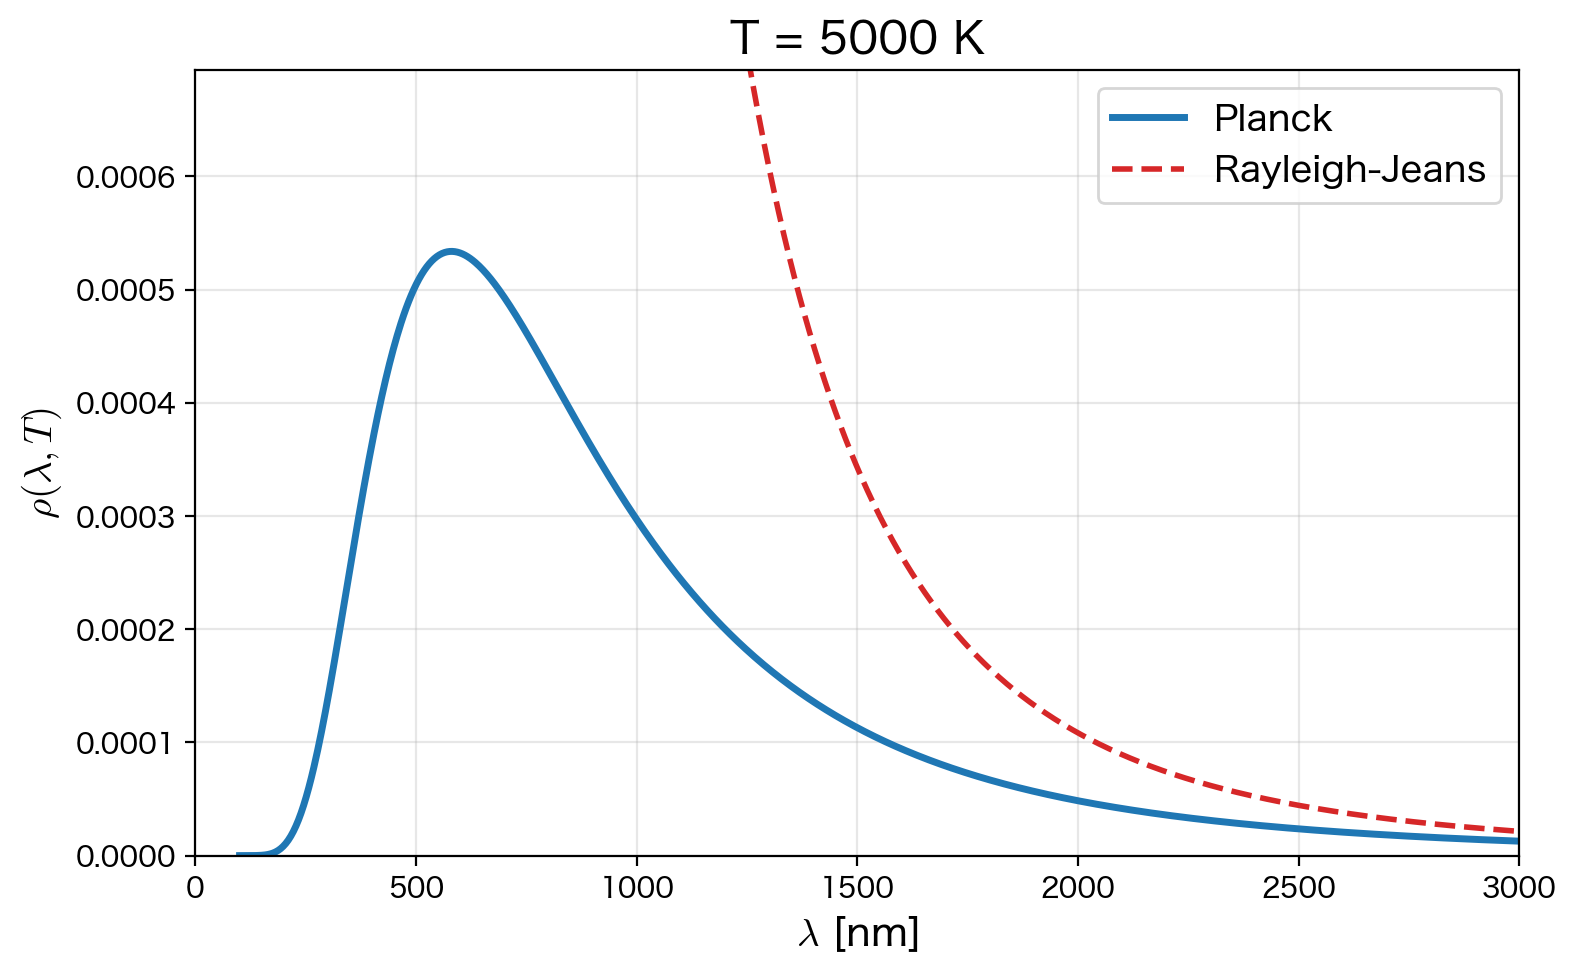
\includegraphics[width=\textwidth]{figures/blackbody.png}
\end{column}
\end{columns}

\end{frame}

\note{
【讲解要点】\\[4pt]
\textbf{背景故事：}19世纪末，物理学家试图用经典力学解释"高温物体为什么会发光"这个问题。\\[4pt]
\textbf{关键矛盾——紫外灾难：}\\
- 经典的瑞利-金斯公式 $\rho = 8\pi k_B T / \lambda^4$\\
- 当波长$\lambda$趋近于0（紫外方向）时，能量密度$\rho$趋向无穷大\\
- 这意味着任何有温度的物体都会辐射出无穷大的能量——显然荒谬！\\
- 实验上，短波长处$\rho$是下降的，不是发散的\\[4pt]
\textbf{看图说话：}右边的图中，虚线是经典理论（发散），实线是实验结果（有峰值后下降）。\\[4pt]
\textbf{过渡：}经典力学在这里彻底失败了，需要全新的想法——这就引出了普朗克的量子假说。
}

% ============================================================
\begin{frame}{Planckの革命的アイデア}

\textbf{Planck (1900)} はこの矛盾を解決するために，\\
古典論の常識を捨てて，大胆な仮定を置きました：

\vspace{0.6em}
\importantbox{
  \textbf{Planckの量子仮説：}\\[4pt]
  電磁波のエネルギーは連続的ではなく，\\
  $h\nu$（$h$：Planck定数，$\nu$：振動数）の\alert{整数倍}でしか取れない。
  \[
    E = nh\nu \qquad (n = 1, 2, 3, \ldots)
  \]
}

\vspace{0.3em}
$h = \SI{6.626e-34}{J.s}$（Planck定数）：とてつもなく小さい値

\vspace{0.3em}
\teacher{日常のスケールでは$h$が小さすぎて量子化に気づかない。\\
原子・分子のスケールで初めて効いてくる。}
\end{frame}

\note{
【讲解要点】\\[4pt]
\textbf{普朗克的革命性想法（1900年）：}\\
- 经典物理认为能量是\textbf{连续}的，可以取任意值\\
- 普朗克说：不！电磁波的能量只能是 $h\nu$ 的整数倍，是"一份一份"的\\
- $h = 6.626 \times 10^{-34}$ J·s，这个数极其小\\[4pt]
\textbf{为什么日常感觉不到量子化？}\\
- 因为$h$太小了。比如你拍一下手释放的能量，对应的量子数$n$是天文数字\\
- 只有在原子、分子尺度（能量极小时），"一份一份"才会被感知到\\[4pt]
\textbf{类比帮助理解：}\\
- 想象上楼梯（能量量子化）vs 上斜坡（能量连续）\\
- 普朗克说：自然界其实是楼梯，只是台阶太小，我们以为是斜坡\\[4pt]
\textbf{入试考点：}记住$E = nh\nu$和$h$的数值。
}

% ============================================================
\begin{frame}{光電効果：光は粒子でもある}

次に，\textbf{Einstein (1905)} がPlanckのアイデアをさらに推し進めました。

\begin{columns}[c]
\begin{column}{0.55\textwidth}
金属に光を当てると電子が飛び出す（\textbf{光電効果}）。

\vspace{0.3em}
\textbf{古典論の予測：}光を強くすれば電子は出るはず\\
\textbf{実験事実：}光の振動数$\nu$が閾値以下なら，\\
\hspace{3em}どんなに強くしても電子は\alert{出ない}

\vspace{0.3em}
\teacher{Einsteinの説明：光は$h\nu$のエネルギーを持つ粒（\textbf{光子}）である。}

\[
  E_\text{kinetic} = h\nu - W
\]
{\small $W$：仕事関数（金属から電子を引き離すのに必要なエネルギー）}
\end{column}
\begin{column}{0.45\textwidth}
  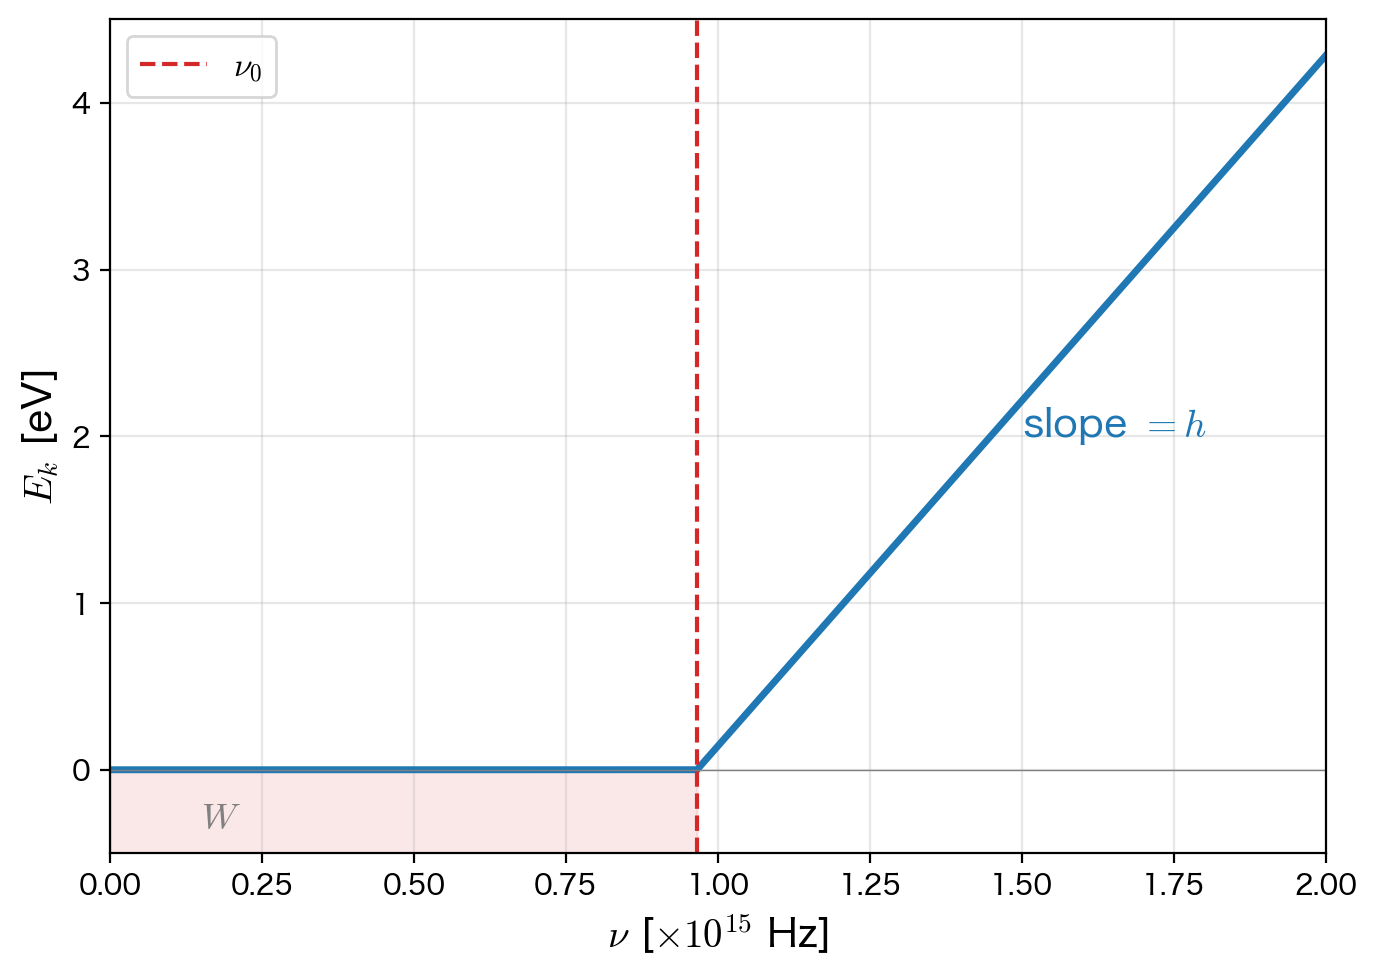
\includegraphics[width=\textwidth]{figures/photoelectric.png}
\end{column}
\end{columns}

\end{frame}

\note{
【讲解要点】\\[4pt]
\textbf{光电效应——爱因斯坦（1905年）：}\\
- 实验现象：光照射金属表面，电子被打出来\\
- 经典预测：光越强（振幅大），电子应该越容易出来\\
- 实验事实：频率$\nu$低于某个阈值时，\textbf{无论光多强都打不出电子}！\\[4pt]
\textbf{爱因斯坦的解释：}\\
- 光不是连续的波，而是一颗颗"光子"，每个光子能量 = $h\nu$\\
- 光子打到电子上，如果 $h\nu < W$（功函数），能量不够，电子出不来\\
- 如果 $h\nu > W$，多余的能量变成电子的动能：$E_k = h\nu - W$\\[4pt]
\textbf{关键理解：}\\
- 增加光强 = 增加光子数量，但每个光子能量不变\\
- 增加频率 = 增加每个光子的能量\\
- 所以频率不够就是打不出电子，跟光强无关\\[4pt]
\textbf{过渡：}光具有粒子性（光子）。那反过来，粒子（如电子）是否也有波动性呢？→ 德布罗意
}

% ============================================================
\begin{frame}{粒子の波動性：ド・ブロイ波}

ここまでで，\textbf{光}は波でもあり粒子でもあることが分かりました。

\vspace{0.3em}
\textbf{de Broglie (1924)} は逆を考えました：

\importantbox{
  光が波と粒子の二重性を持つなら，\\
  \textbf{粒子}（電子など）も波としての性質を持つのではないか？
  \[
    \lambda = \frac{h}{p} = \frac{h}{mv} \qquad \text{（ド・ブロイ波長）}
  \]
}

\vspace{0.3em}
{\small 電子線回折実験 (Davisson--Germer, 1927) で実証。}

\teacher{粒子が波なら，その波を記述する方程式が必要 → Schrödinger方程式へ。}
\end{frame}

\note{
【讲解要点】\\[4pt]
\textbf{德布罗意的逆向思维（1924年）：}\\
- 前面我们知道了：光（传统上认为是波）其实也是粒子（光子）\\
- 德布罗意反过来想：既然波有粒子性，那粒子是否也有波动性？\\
- 他提出：任何粒子都有一个对应的波长 $\lambda = h/p = h/(mv)$\\[4pt]
\textbf{物理直觉：}\\
- 质量越大、速度越快 → 动量$p$越大 → 波长$\lambda$越短\\
- 宏观物体（比如棒球）的$\lambda$小到可以忽略，所以看不到波动性\\
- 电子很轻，$\lambda$可以达到原子尺度，波动性就很明显了\\[4pt]
\textbf{实验验证：}1927年戴维森-革末实验，电子束打到镍晶体上，出现了衍射图样——跟X射线衍射一样！证明电子确实是波。\\[4pt]
\textbf{逻辑链条总结：}\\
黑体辐射（能量量子化）→ 光电效应（光是粒子）→ 德布罗意（粒子是波）→ 需要描述"粒子波"的方程 → 薛定谔方程！
}

% %%%%%%%%%%%%%%%%%%%%%%%%%%%%%%%%%%%%%%%%%%%%%%%%%%%%%%%%%%%%
\section{Schrödinger方程式はどこから来るのか}
% %%%%%%%%%%%%%%%%%%%%%%%%%%%%%%%%%%%%%%%%%%%%%%%%%%%%%%%%%%%%

% ============================================================
\begin{frame}{出発点：粒子を波として書く}

粒子が波なら，波の式（\textbf{波動関数}）で書けるはずです。

\vspace{0.3em}
一般的な平面波：
\[
  \Psi(x,t) = A \exp\!\left[2\pi i\!\left(\frac{x}{\lambda} - \nu t\right)\right]
\]

ここに de Broglie の関係（$\lambda = h/p$，$E = h\nu$）を代入すると：

\[
  \lambda = \frac{h}{p} = \frac{2\pi\hbar}{p}, \qquad
  \nu = \frac{E}{h}
\]

\importantbox{
  $\displaystyle \Psi(x,t) = A \exp\!\left[\frac{i}{\hbar}(px - Et)\right]$
}

{\small $\hbar \equiv h/(2\pi)$：ディラック定数（換算Planck定数）}

\vspace{0.3em}
\teacher{この式が全ての出発点です。ここから微分で演算子を導きます。}
\end{frame}

\note{
【讲解要点】\\[4pt]
\textbf{从平面波出发：}\\
- 既然粒子是波，我们就用波的数学表达式来描述它\\
- 一般的平面波：$\Psi = A \exp[2\pi i(x/\lambda - \nu t)]$\\
- 把德布罗意关系 $\lambda = h/p$ 和 $E = h\nu$ 代入\\
- 得到：$\Psi = A \exp[\frac{i}{\hbar}(px - Et)]$\\[4pt]
\textbf{$\hbar$是什么？}\\
- $\hbar = h/(2\pi)$，叫"约化普朗克常数"或"狄拉克常数"\\
- 在量子力学中$\hbar$比$h$用得更多，因为公式更简洁\\[4pt]
\textbf{这个式子为什么重要？}\\
- 它把粒子的物理量（动量$p$、能量$E$）和波函数联系起来了\\
- 接下来我们会发现：对这个波函数求导，就能"提取"出$p$和$E$\\
- 这就是量子力学中"算符"概念的起源\\[4pt]
\textbf{过渡：}下一页我们来看，对$x$求导为什么能得到动量。
}

% ============================================================
\begin{frame}{なぜ微分すると運動量が出るのか}

$\Psi = A\exp\!\bigl[\tfrac{i}{\hbar}(px - Et)\bigr]$ を$x$で偏微分してみましょう：

\[
  \frac{\partial \Psi}{\partial x}
  = A \cdot \frac{ip}{\hbar} \cdot \exp\!\left[\frac{i}{\hbar}(px - Et)\right]
  = \frac{ip}{\hbar}\,\Psi
\]

両辺に$\dfrac{\hbar}{i}$をかけると：

\[
  \frac{\hbar}{i}\frac{\partial \Psi}{\partial x} = p\,\Psi
\]

\teacher{$x$で微分するという「操作」が，$p$という「値」を取り出した！\\
このような操作を\textbf{演算子}，取り出された値を\textbf{固有値}と呼びます。}

\importantbox{
  \textbf{運動量演算子：}\quad $\hat{p} = \dfrac{\hbar}{i}\dfrac{\partial}{\partial x} = -i\hbar\dfrac{\partial}{\partial x}$
}
\end{frame}

\note{
【讲解要点】\\[4pt]
\textbf{推导过程（一定要慢慢讲清楚）：}\\
1. 把 $\Psi = A\exp[\frac{i}{\hbar}(px-Et)]$ 对$x$求偏导\\
2. 指数函数求导，系数 $\frac{ip}{\hbar}$ 跑出来，指数部分不变\\
3. 所以 $\frac{\partial\Psi}{\partial x} = \frac{ip}{\hbar}\Psi$\\
4. 两边乘以 $\frac{\hbar}{i}$，得到 $\frac{\hbar}{i}\frac{\partial\Psi}{\partial x} = p\Psi$\\[4pt]
\textbf{关键概念——算符与本征值：}\\
- "对$x$求导再乘$\hbar/i$"这个\textbf{操作}叫做\textbf{算符}（operator），记作$\hat{p}$\\
- 操作作用在$\Psi$上，得到的是一个\textbf{数}（$p$）乘以$\Psi$本身\\
- 这个数$p$叫做\textbf{本征值}（eigenvalue），$\Psi$叫\textbf{本征函数}（eigenfunction）\\
- 这就是量子力学的核心数学结构：$\hat{A}\psi = a\psi$\\[4pt]
\textbf{动量算符：}$\hat{p} = -i\hbar\frac{\partial}{\partial x}$\\[4pt]
\textbf{入试提示：}这个推导经常作为"请导出动量算符"的题目出现。
}

% ============================================================
\begin{frame}{同様に，エネルギー演算子}

今度は$t$で偏微分してみます：

\[
  \frac{\partial \Psi}{\partial t}
  = A \cdot \frac{(-iE)}{\hbar} \cdot \exp\!\left[\frac{i}{\hbar}(px - Et)\right]
  = \frac{-iE}{\hbar}\,\Psi
\]

整理すると：

\[
  i\hbar\frac{\partial \Psi}{\partial t} = E\,\Psi
\]

\importantbox{
  \textbf{エネルギー演算子：}\quad $\hat{E} = i\hbar\dfrac{\partial}{\partial t}$
}

\vspace{0.3em}
\teacher{まとめると：\\
$x$で微分 → 運動量$p$が出る　／　$t$で微分 → エネルギー$E$が出る\\
これが量子力学の\textbf{演算子と固有値}の考え方です。}
\end{frame}

\note{
【讲解要点】\\[4pt]
\textbf{同样的思路，对$t$求导：}\\
1. $\frac{\partial\Psi}{\partial t} = \frac{-iE}{\hbar}\Psi$（注意负号，因为指数中$t$前面是$-E$）\\
2. 两边乘以$i\hbar$：$i\hbar\frac{\partial\Psi}{\partial t} = E\Psi$\\
3. 所以能量算符是 $\hat{E} = i\hbar\frac{\partial}{\partial t}$\\[4pt]
\textbf{总结对比：}\\
- 对$x$求导 → 提取动量$p$ → 动量算符 $\hat{p} = -i\hbar\partial_x$\\
- 对$t$求导 → 提取能量$E$ → 能量算符 $\hat{E} = i\hbar\partial_t$\\[4pt]
\textbf{深层理解：}\\
在量子力学中，物理量不再是"数"，而是"操作"（算符）。\\
测量一个物理量 = 让对应的算符作用在波函数上。\\
这是量子力学和经典力学最根本的区别之一。\\[4pt]
\textbf{过渡：}现在我们有了动量算符和能量算符，下一步就是把经典力学的能量关系$E = p^2/(2m) + V$中的$p$和$E$替换成算符，得到薛定谔方程。
}

% ============================================================
\begin{frame}{Schrödinger方程式の完成}

古典力学：$E = p^2/(2m) + V(x)$ に演算子を代入：

$p \to \hat{p} = -i\hbar\partial_x$，\;$E \to \hat{E} = i\hbar\partial_t$

\[
  \hat{H} = -\frac{\hbar^2}{2m}\frac{\partial^2}{\partial x^2} + V(x)
  \quad \text{（\textbf{ハミルトニアン}：全エネルギーの演算子）}
\]

\importantbox{
  \textbf{時間依存Schrödinger方程式：}\;
  $\displaystyle \hat{H}\Psi = i\hbar\frac{\partial}{\partial t}\Psi$
}

\teacher{量子力学の全てはこの1本の方程式から出発します。}
\end{frame}

\note{
【讲解要点】\\[4pt]
\textbf{薛定谔方程的"推导"：}\\
- 经典力学的能量守恒：$E = \frac{p^2}{2m} + V(x)$（动能+势能）\\
- 把$p$换成$\hat{p} = -i\hbar\partial_x$，$E$换成$\hat{E} = i\hbar\partial_t$\\
- $p^2/(2m) \to \hat{p}^2/(2m) = (-i\hbar\partial_x)^2/(2m) = -\frac{\hbar^2}{2m}\partial_x^2$\\
- 左边的总能量算符叫\textbf{哈密顿量}（Hamiltonian）$\hat{H}$\\[4pt]
\textbf{哈密顿量 $\hat{H}$ 的组成：}\\
$\hat{H} = \underbrace{-\frac{\hbar^2}{2m}\frac{\partial^2}{\partial x^2}}_{\text{动能算符}} + \underbrace{V(x)}_{\text{势能}}$\\[4pt]
\textbf{薛定谔方程：}$\hat{H}\Psi = i\hbar\frac{\partial\Psi}{\partial t}$\\[4pt]
\textbf{重要说明：}薛定谔方程不是"推导"出来的，它是一个\textbf{公设}（postulate）。上面的过程只是启发性的，帮助理解它的由来。\\[4pt]
\textbf{过渡：}这是含时薛定谔方程。但入试中更常用的是不含时的版本，下面来看怎么分离变量。
}

% ============================================================
\begin{frame}{時間に依存しないSchrödinger方程式}

$V(x)$が時間に依存しない場合，変数分離$\Psi = \psi(x)\cdot T(t)$で：
\[
  \underbrace{\frac{1}{\psi}\hat{H}\psi}_{x\text{のみ}}
  = \underbrace{\frac{i\hbar}{T}\frac{dT}{dt}}_{t\text{のみ}}
  = E \quad (\text{定数})
\]

\importantbox{
  \textbf{時間非依存Schrödinger方程式：}\;
  $\displaystyle -\frac{\hbar^2}{2m}\frac{d^2\psi}{dx^2} + V(x)\psi = E\psi$
}

時間部分：$T(t) = e^{-iEt/\hbar}$，全体：$\Psi(x,t) = \psi(x)\,e^{-iEt/\hbar}$

\teacher{入試で「Schrödinger方程式を書け」＝ ほぼこの時間非依存形のこと。}
\end{frame}

\note{
【讲解要点】\\[4pt]
\textbf{变量分离法：}\\
- 假设$V(x)$不随时间变化（定态问题）\\
- 设 $\Psi(x,t) = \psi(x) \cdot T(t)$，把空间和时间分开\\
- 代入含时薛定谔方程，左边只含$x$，右边只含$t$\\
- 一个只关于$x$的表达式等于一个只关于$t$的表达式，那两边都必须等于同一个常数$E$\\[4pt]
\textbf{两个方程：}\\
- 空间部分：$\hat{H}\psi = E\psi$（这就是\textbf{定态薛定谔方程}）\\
- 时间部分：$i\hbar\frac{dT}{dt} = ET$，解为 $T(t) = e^{-iEt/\hbar}$\\[4pt]
\textbf{入试最重要的公式：}\\
$-\frac{\hbar^2}{2m}\frac{d^2\psi}{dx^2} + V(x)\psi = E\psi$\\[4pt]
\textbf{提醒：}考试说"写出薛定谔方程"，99\%指的是这个定态版本。\\[4pt]
\textbf{过渡：}方程有了，怎么解？先用一个更简单的例子——弦的振动方程——来练习变量分离法。
}

% %%%%%%%%%%%%%%%%%%%%%%%%%%%%%%%%%%%%%%%%%%%%%%%%%%%%%%%%%%%%
\section{どうやって解くのか（変数分離法）}
% %%%%%%%%%%%%%%%%%%%%%%%%%%%%%%%%%%%%%%%%%%%%%%%%%%%%%%%%%%%%

% ============================================================
\begin{frame}{数学の準備：なぜ波動方程式を先に学ぶのか}

Schrödinger方程式は\textbf{二階偏微分方程式}の一種です。

\vspace{0.3em}
\teacher{解き方のパターンを掴むために，\\
もっと馴染みのある\textbf{弦の振動}（波動方程式）で練習しましょう。\\
解法の手順はSchrödinger方程式と\alert{全く同じ}です。}

\vspace{0.3em}
\textbf{波動方程式：}
\[
  \frac{\partial^2 u}{\partial t^2} = c^2 \frac{\partial^2 u}{\partial x^2}
  \qquad (0 < x < L)
\]

\textbf{解法の手順：}
\begin{enumerate}
  \item $u(x,t) = f(x)\cdot g(t)$ と置く（\textbf{変数分離}）
  \item $x$だけの式と$t$だけの式に分離 → 各々を常微分方程式として解く
  \item \textbf{境界条件}を適用 → 解の形が確定
  \item 許されるエネルギー（固有値）が\alert{離散的}に決まる
\end{enumerate}
\end{frame}

\note{
【讲解要点】\\[4pt]
\textbf{为什么先讲波动方程？}\\
- 薛定谔方程是二阶偏微分方程，数学上跟弦的振动方程是同一类\\
- 弦振动更直观，先拿它练手，掌握解题套路\\
- 然后把完全相同的套路用到薛定谔方程上\\[4pt]
\textbf{解题四步走（万能套路）：}\\
1. \textbf{变量分离}：设$u = f(x) \cdot g(t)$\\
2. \textbf{分离方程}：代入后分成只含$x$和只含$t$的两个方程\\
3. \textbf{施加边界条件}：比如弦两端固定 → $f(0)=0$, $f(L)=0$\\
4. \textbf{得到离散解}：不是所有的$E$都行，只有特定的值才满足边界条件\\[4pt]
\textbf{强调：}这四步在后面解井戸型势时会\textbf{原封不动}地再用一次！\\[4pt]
\textbf{过渡：}下面来执行变量分离，看看具体怎么做。
}

% ============================================================
\begin{frame}{変数分離の実行}

$u = f(x)g(t)$ を波動方程式に代入して，両辺を$f\cdot g$で割ると：

\[
  \frac{1}{c^2 g}\frac{d^2 g}{dt^2}
  = \frac{1}{f}\frac{d^2 f}{dx^2}
\]

\teacher{左辺は$t$だけ，右辺は$x$だけの関数です。\\
$x$と$t$は独立に動くのに等式が成り立つ → \alert{両辺は定数}でなければならない。}

\vspace{0.3em}
この定数を$\lambda$と置くと，$x$部分だけ取り出せます：

\importantbox{
  $\dfrac{d^2 f}{dx^2} = \lambda f(x)$
  \quad ← 二階の常微分方程式（\textbf{固有値問題}）
}

\teacher{$\lambda$の値によって解の形が全く変わります。\\
次のスライドで場合分けを見ましょう。}
\end{frame}

\note{
【讲解要点】\\[4pt]
\textbf{变量分离的关键逻辑：}\\
- 代入$u = f(x)g(t)$后，左边只含$t$，右边只含$x$\\
- $x$和$t$是\textbf{独立}变量，各自可以随意变化\\
- 如果一个只含$t$的函数恒等于一个只含$x$的函数，那两边都必须是\textbf{常数}\\
- 这个常数我们叫$\lambda$（分离常数）\\[4pt]
\textbf{得到的方程：}$f'' = \lambda f$\\
- 这是一个二阶常微分方程（ODE），比偏微分方程（PDE）好解多了\\
- 这就是变量分离法的威力：把PDE变成ODE\\[4pt]
\textbf{$\lambda$的值怎么确定？}\\
- 不是随便取的！要靠边界条件来限定\\
- 下一页讨论$\lambda > 0$、$\lambda = 0$、$\lambda < 0$三种情况
}

% ============================================================
\begin{frame}{$\lambda$の符号で解が決まる}

\begin{columns}[T]
\begin{column}{0.5\textwidth}
  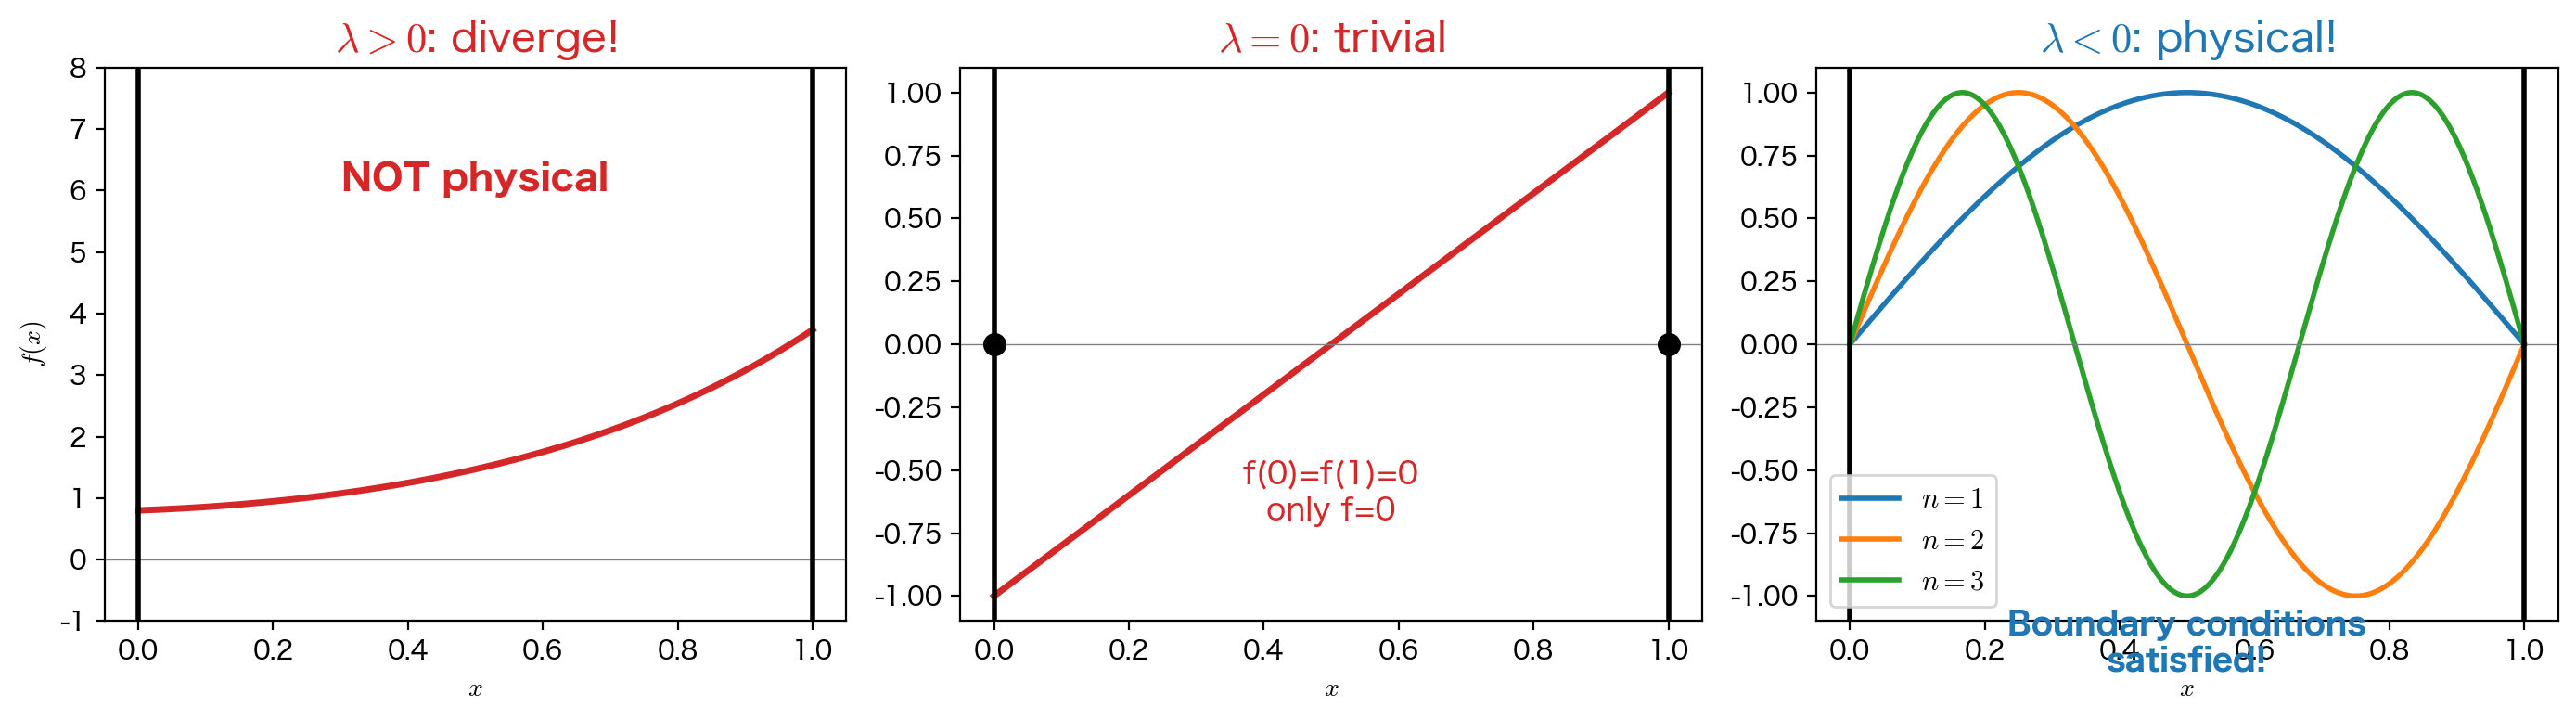
\includegraphics[width=0.95\textwidth]{figures/lambda_cases.png}
\end{column}
\begin{column}{0.5\textwidth}
\textbf{\color{alertred}$\lambda > 0$：}
指数関数 → 発散 → \textbf{不適}

\vspace{0.3em}
\textbf{\color{alertred}$\lambda = 0$：}
直線 → 自明解のみ → \textbf{不適}

\vspace{0.3em}
\textbf{\color{darkblue}$\lambda < 0$：}
三角関数（$\sin$, $\cos$）→ 境界条件を満たせる！
\end{column}
\end{columns}

\vspace{0.3em}
\teacher{$\lambda < 0$のみ物理的に正しい。}
境界条件$f(0) = 0$, $f(L) = 0$を適用：
\[
  \boxed{f_n(x) = D\sin\!\left(\frac{n\pi x}{L}\right), \quad n = 1,2,3,\ldots}
\]
\end{frame}

\note{
【讲解要点】\\[4pt]
\textbf{三种情况的分析（对$f'' = \lambda f$）：}\\[4pt]
\textbf{1. $\lambda > 0$（设$\lambda = k^2$）：}\\
- 解是指数函数：$f = Ae^{kx} + Be^{-kx}$\\
- 指数函数会发散到无穷大，不满足边界条件 → 排除\\[4pt]
\textbf{2. $\lambda = 0$：}\\
- 解是直线：$f = Ax + B$\\
- 边界条件$f(0)=0$, $f(L)=0$ → $A=B=0$，只有零解 → 没意义\\[4pt]
\textbf{3. $\lambda < 0$（设$\lambda = -k^2$）：}\\
- 解是三角函数：$f = A\cos(kx) + B\sin(kx)$\\
- $f(0) = 0$ → $A = 0$，只剩$\sin$\\
- $f(L) = 0$ → $\sin(kL) = 0$ → $kL = n\pi$\\
- 最终：$f_n(x) = D\sin(n\pi x / L)$\\[4pt]
\textbf{重要结论：}边界条件把连续的参数$k$限制为离散的$n\pi/L$，这就是量子化的数学根源！\\[4pt]
\textbf{看图：}左边的图清楚展示了三种解的形状。
}

% %%%%%%%%%%%%%%%%%%%%%%%%%%%%%%%%%%%%%%%%%%%%%%%%%%%%%%%%%%%%
\section{井戸型ポテンシャル（Particle in a Box）}
% %%%%%%%%%%%%%%%%%%%%%%%%%%%%%%%%%%%%%%%%%%%%%%%%%%%%%%%%%%%%

% ============================================================
\begin{frame}{箱の中の粒子（Particle in a Box）}

\begin{columns}[c]
\begin{column}{0.4\textwidth}
  \begin{tikzpicture}[scale=0.75]
    \fill[pattern=north east lines, pattern color=gray] (-0.5,0) rectangle (0,2.5);
    \fill[pattern=north east lines, pattern color=gray] (3.5,0) rectangle (4,2.5);
    \draw[very thick] (0,2.5) -- (0,0) -- (3.5,0) -- (3.5,2.5);
    \fill[yellow!30, opacity=0.5] (0,0) rectangle (3.5,2.5);
    \node[below] at (0,-0.1) {\small$0$};
    \node[below] at (3.5,-0.1) {\small$a$};
    \node at (1.75,1.2) {$V=0$};
    \node at (-0.8,1.2) {\small$\infty$};
    \node at (4.3,1.2) {\small$\infty$};
  \end{tikzpicture}
\end{column}
\begin{column}{0.6\textwidth}
  $V(x) = 0\;(0 \leq x \leq a)$，それ以外$V = \infty$

  壁の外：$\psi = 0$（存在確率ゼロ）

  \vspace{0.3em}
  箱の中（$V = 0$）のSchrödinger方程式：
  \[
    -\frac{\hbar^2}{2m}\frac{d^2\psi}{dx^2} = E\psi
  \]
\end{column}
\end{columns}

$k \equiv \sqrt{2mE/\hbar^2}$ とおくと：
\[
  \frac{d^2\psi}{dx^2} = -k^2\psi
\]

\teacher{波動方程式で練習した$f'' = \lambda f$（$\lambda = -k^2$）と\alert{全く同じ形}！}
\end{frame}

\note{
【讲解要点】\\[4pt]
\textbf{模型设定——无限深方势阱：}\\
- 想象一个粒子被关在一个"箱子"里\\
- 箱子内（$0 \leq x \leq a$）：势能$V = 0$，粒子自由运动\\
- 箱子外：势能$V = \infty$，粒子绝对出不去，$\psi = 0$\\
- 这是量子力学最基本、最重要的模型！\\[4pt]
\textbf{方程简化：}\\
- 箱内$V = 0$，薛定谔方程变为：$-\frac{\hbar^2}{2m}\psi'' = E\psi$\\
- 令$k = \sqrt{2mE/\hbar^2}$，得到 $\psi'' = -k^2\psi$\\
- 这跟我们刚才练习的弦振动方程\textbf{一模一样}！\\[4pt]
\textbf{强调与弦振动的平行关系：}\\
- 弦振动：两端固定 → $f(0) = f(L) = 0$\\
- 箱中粒子：两壁处$\psi = 0$ → $\psi(0) = \psi(a) = 0$\\
- 解法完全一样！\\[4pt]
\textbf{过渡：}套路已经熟悉了，现在来施加边界条件。
}

% ============================================================
\begin{frame}{境界条件の適用}

一般解：$\psi(x) = A\cos(kx) + B\sin(kx)$

\vspace{0.3em}
\textbf{境界条件①：} $\psi(0) = 0$
\[
  \psi(0) = A\cos(0) + B\sin(0) = A = 0
\]

\teacher{$A = 0$なので，$\psi(x) = B\sin(kx)$だけが残ります。}

\vspace{0.3em}
\textbf{境界条件②：} $\psi(a) = 0$
\[
  \psi(a) = B\sin(ka) = 0
\]

$B = 0$だと$\psi = 0$（粒子が存在しない）→ 意味がないので$B \neq 0$。\\
したがって：
\[
  \sin(ka) = 0 \quad \Longrightarrow \quad ka = n\pi \quad (n = 1, 2, 3, \ldots)
\]

\importantbox{
  $k = \dfrac{n\pi}{a}$，\qquad $\psi_n(x) = B\sin\!\left(\dfrac{n\pi x}{a}\right)$
}

{\small ※ $n = 0$は$\psi = 0$（粒子不存在）なので除外。}
\end{frame}

\note{
【讲解要点】\\[4pt]
\textbf{施加边界条件（逐步推导）：}\\[4pt]
\textbf{步骤1：}一般解 $\psi = A\cos(kx) + B\sin(kx)$\\[4pt]
\textbf{步骤2：}左边界 $\psi(0) = 0$\\
- $A\cos(0) + B\sin(0) = A \cdot 1 + B \cdot 0 = A = 0$\\
- 所以$\cos$项消失，$\psi = B\sin(kx)$\\[4pt]
\textbf{步骤3：}右边界 $\psi(a) = 0$\\
- $B\sin(ka) = 0$\\
- $B \neq 0$（否则粒子不存在），所以必须 $\sin(ka) = 0$\\
- $\sin$什么时候等于零？$ka = n\pi$（$n = 1, 2, 3, \ldots$）\\
- 注意$n = 0$排除，因为那样$\psi$处处为零\\[4pt]
\textbf{关键结论：}\\
- $k$不是可以连续变化的，只能取$n\pi/a$这些离散值\\
- 这就是\textbf{量子化}！边界条件自然地导致了能量只能取离散值\\[4pt]
\textbf{过渡：}波函数的形状确定了，但系数$B$还没定。下面用归一化来确定$B$。
}

% ============================================================
\begin{frame}{規格化：係数$B$を決める}

\teacher{「粒子がどこかに必ず存在する」→ 確率の総和$= 1$で$B$が決まる。}

\[
  \int_0^a |\psi_n|^2\,dx = B^2 \int_0^a \sin^2\!\left(\frac{n\pi x}{a}\right)dx = 1
\]

半角公式 $\sin^2\theta = (1 - \cos 2\theta)/2$ で積分：
\[
  B^2 \int_0^a \frac{1 - \cos(2n\pi x/a)}{2}\,dx
  = B^2 \left[\frac{x}{2} - \frac{a}{4n\pi}\sin\!\left(\frac{2n\pi x}{a}\right)\right]_0^a
  = B^2 \cdot \frac{a}{2}
\]

$\therefore\; B = \sqrt{2/a}$

\importantbox{
  $\boxed{\psi_n(x) = \sqrt{\dfrac{2}{a}}\sin\!\left(\dfrac{n\pi x}{a}\right), \quad n = 1, 2, 3, \ldots}$
}
\end{frame}

\note{
【讲解要点】\\[4pt]
\textbf{归一化的物理含义：}\\
- 粒子总得在箱子里的\textbf{某个地方}，所以找到它的总概率必须等于1\\
- $\int_0^a |\psi|^2 dx = 1$\\[4pt]
\textbf{积分技巧（半角公式）：}\\
- $\sin^2\theta = \frac{1 - \cos 2\theta}{2}$，这是入试必须记住的公式\\
- $\int_0^a \sin^2(n\pi x/a) dx = a/2$（$\cos$项积分后在$[0,a]$上为零）\\
- 所以 $B^2 \cdot a/2 = 1$，$B = \sqrt{2/a}$\\[4pt]
\textbf{最终结果（必背公式）：}\\
$\psi_n(x) = \sqrt{\frac{2}{a}}\sin\left(\frac{n\pi x}{a}\right)$，$n = 1, 2, 3, \ldots$\\[4pt]
\textbf{入试考点：}\\
- "请对箱中粒子的波函数进行归一化"是经典题目\\
- 一定要记住半角公式和最终结果
}

% ============================================================
\begin{frame}{エネルギー固有値}

$k = \sqrt{2mE/\hbar^2} = n\pi/a$ から$E$について解くと：

\importantbox{
  \[
    \boxed{E_n = \frac{n^2\pi^2\hbar^2}{2ma^2} = \frac{n^2 h^2}{8ma^2}, \qquad n = 1, 2, 3, \ldots}
  \]
}

\teacher{エネルギーは連続ではなく，$n = 1, 2, 3, \ldots$の\alert{飛び飛びの値}しか取れません。}

\vspace{0.3em}
\begin{center}
\begin{tabular}{lcc}
  \toprule
  & \textbf{古典力学} & \textbf{量子力学} \\
  \midrule
  エネルギー & 連続（任意の値） & \alert{離散的}（$n^2$に比例） \\
  最低エネルギー & $E = 0$（静止可能） & $E_1 > 0$（\alert{零点エネルギー}） \\
  \bottomrule
\end{tabular}
\end{center}
\end{frame}

\note{
【讲解要点】\\[4pt]
\textbf{能量本征值的推导：}\\
- 从 $k = \sqrt{2mE/\hbar^2} = n\pi/a$\\
- 两边平方：$2mE/\hbar^2 = n^2\pi^2/a^2$\\
- 解出$E$：$E_n = \frac{n^2\pi^2\hbar^2}{2ma^2}$\\
- 用$\hbar = h/(2\pi)$代入化简：$E_n = \frac{n^2 h^2}{8ma^2}$\\[4pt]
\textbf{两个重要特征：}\\
1. \textbf{能量量子化}：$E$只能取$E_1, 4E_1, 9E_1, 16E_1, \ldots$（$\propto n^2$）\\
2. \textbf{零点能}：最低能量$E_1 \neq 0$，粒子永远不能完全静止\\[4pt]
\textbf{与经典力学的对比：}\\
- 经典：能量连续，最低可以是0（粒子静止不动）\\
- 量子：能量离散，最低是$E_1 > 0$\\[4pt]
\textbf{入试提示：}$E_n = n^2 h^2/(8ma^2)$ 是最高频考点，必须记住！
}

% ============================================================
\begin{frame}{量子効果はどのくらい大きいか}

\textbf{数値例：}電子（$m = \SI{9.11e-31}{kg}$）を$a = \SI{1}{nm}$の箱に入れると
\[
  E_1 = \frac{(\SI{6.626e-34}{})^2}{8 \times \SI{9.11e-31}{} \times (\SI{1e-9}{})^2}
  \approx \SI{0.376}{eV}
\]

室温の熱エネルギー：$k_\mathrm{B}T \approx \SI{0.025}{eV}$

\vspace{0.3em}
\importantbox{
  $E_1 \approx \SI{0.376}{eV} \gg k_\mathrm{B}T \approx \SI{0.025}{eV}$\\[4pt]
  → 原子・分子スケールでは量子効果は\alert{無視できない}！
}

\teacher{逆にマクロな物体（$m$が大きい，$a$が大きい）では$E_1 \approx 0$\\
→ エネルギーが事実上連続 → 古典力学で十分。}
\end{frame}

\note{
【讲解要点】\\[4pt]
\textbf{用数字说话：}\\
- 把一个电子关在1 nm的箱子里（大约原子尺度）\\
- 基态能量$E_1 \approx 0.376$ eV\\
- 室温热能$k_BT \approx 0.025$ eV\\
- $E_1$是$k_BT$的15倍！量子效应完全不能忽略\\[4pt]
\textbf{反过来想（宏观情况）：}\\
- 把一个乒乓球（$m \sim 3$g）关在一个1m的箱子里\\
- $E_1$小到$10^{-65}$ J量级，完全可以忽略\\
- 所以宏观世界用经典力学就够了\\[4pt]
\textbf{什么时候需要量子力学？}\\
- 质量小（电子级别）+ 空间小（nm级别）= 量子效应显著\\
- 这正好是原子和分子的尺度！所以化学离不开量子力学\\[4pt]
\textbf{过渡：}知道了能量和波函数之后，来看它们的物理意义。
}

% %%%%%%%%%%%%%%%%%%%%%%%%%%%%%%%%%%%%%%%%%%%%%%%%%%%%%%%%%%%%
\section{解から何が分かるのか}
% %%%%%%%%%%%%%%%%%%%%%%%%%%%%%%%%%%%%%%%%%%%%%%%%%%%%%%%%%%%%

% ============================================================
\begin{frame}{波動関数の物理的意味（Bornの確率解釈）}

\teacher{$\psi_n(x)$が求まりましたが，これは何を意味するのでしょうか？}

\vspace{0.3em}
\textbf{Born (1926)} の解釈：

\importantbox{
  $|\psi(x)|^2\,dx$ = 位置$x$〜$x + dx$に粒子を見出す\textbf{確率}
}

波動関数が満たすべき条件：
\begin{enumerate}
  \item \textbf{規格化：}$\int|\psi|^2 dx = 1$（どこかに必ずいる）
  \item \textbf{連続：}$\psi(x)$はなめらか
  \item \textbf{一価：}各点で値が一つ
  \item \textbf{有界：}$\psi(x)$は有限
\end{enumerate}

\vspace{0.3em}
\teacher{$\psi$自体は複素数で直接の意味はありませんが，\\
$|\psi|^2$は「粒子をそこで見つける確率」という明確な物理量です。}
\end{frame}

\note{
【讲解要点】\\[4pt]
\textbf{玻恩的概率诠释（1926年）：}\\
- 波函数$\psi(x)$本身是复数，没有直接的物理意义\\
- 但$|\psi(x)|^2$有明确含义：在$x$处找到粒子的\textbf{概率密度}\\
- $|\psi(x)|^2 dx$ = 在$x$到$x+dx$之间找到粒子的概率\\[4pt]
\textbf{波函数必须满足的四个条件：}\\
1. 归一化：总概率=1\\
2. 连续：不能有跳变\\
3. 单值：每个位置只有一个概率\\
4. 有界：不能发散到无穷大\\[4pt]
\textbf{容易搞混的点：}\\
- $\psi$可以是负的（比如$\sin$函数），但$|\psi|^2$一定$\geq 0$（概率不能为负）\\
- $\psi$有"节点"（零点），意味着粒子在那个位置的概率为零\\[4pt]
\textbf{过渡：}来看看波函数和概率密度长什么样。
}

% ============================================================
\begin{frame}{波動関数と存在確率を見てみよう}

\begin{columns}[T]
\begin{column}{0.5\textwidth}
  \centering
  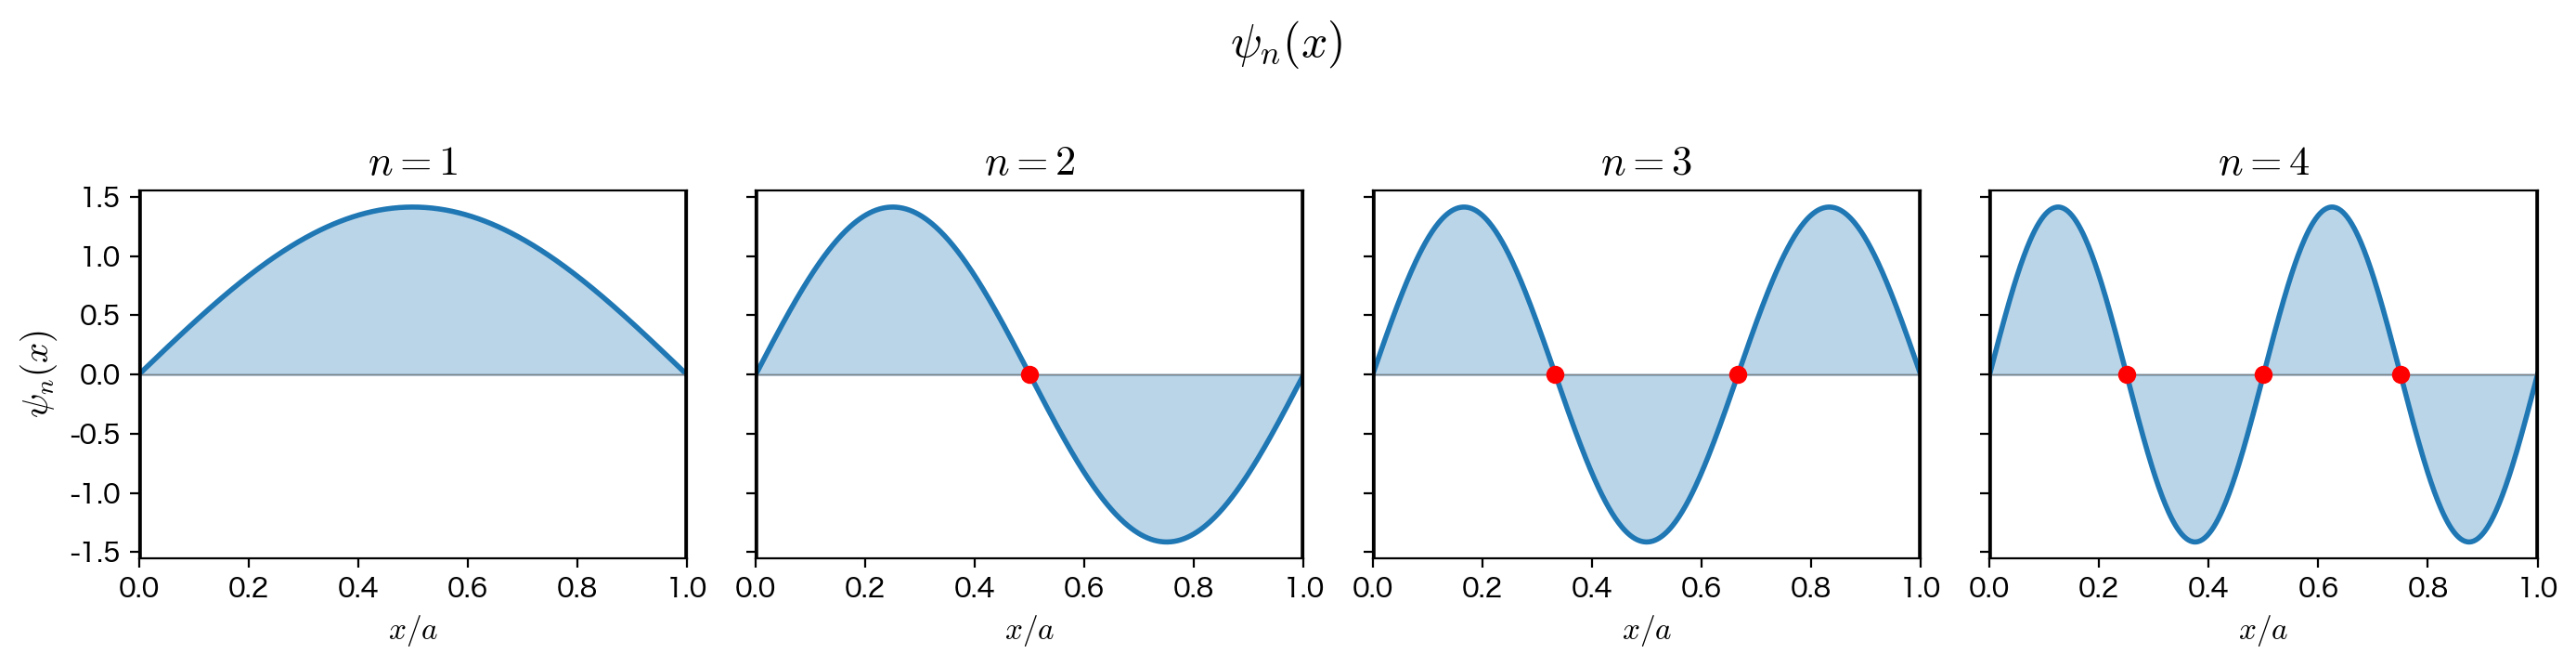
\includegraphics[width=\textwidth]{figures/wavefunctions.png}\\
  {\small $\psi_n(x)$：赤丸＝\textbf{節}（$\psi = 0$の点）}
\end{column}
\begin{column}{0.5\textwidth}
  \centering
  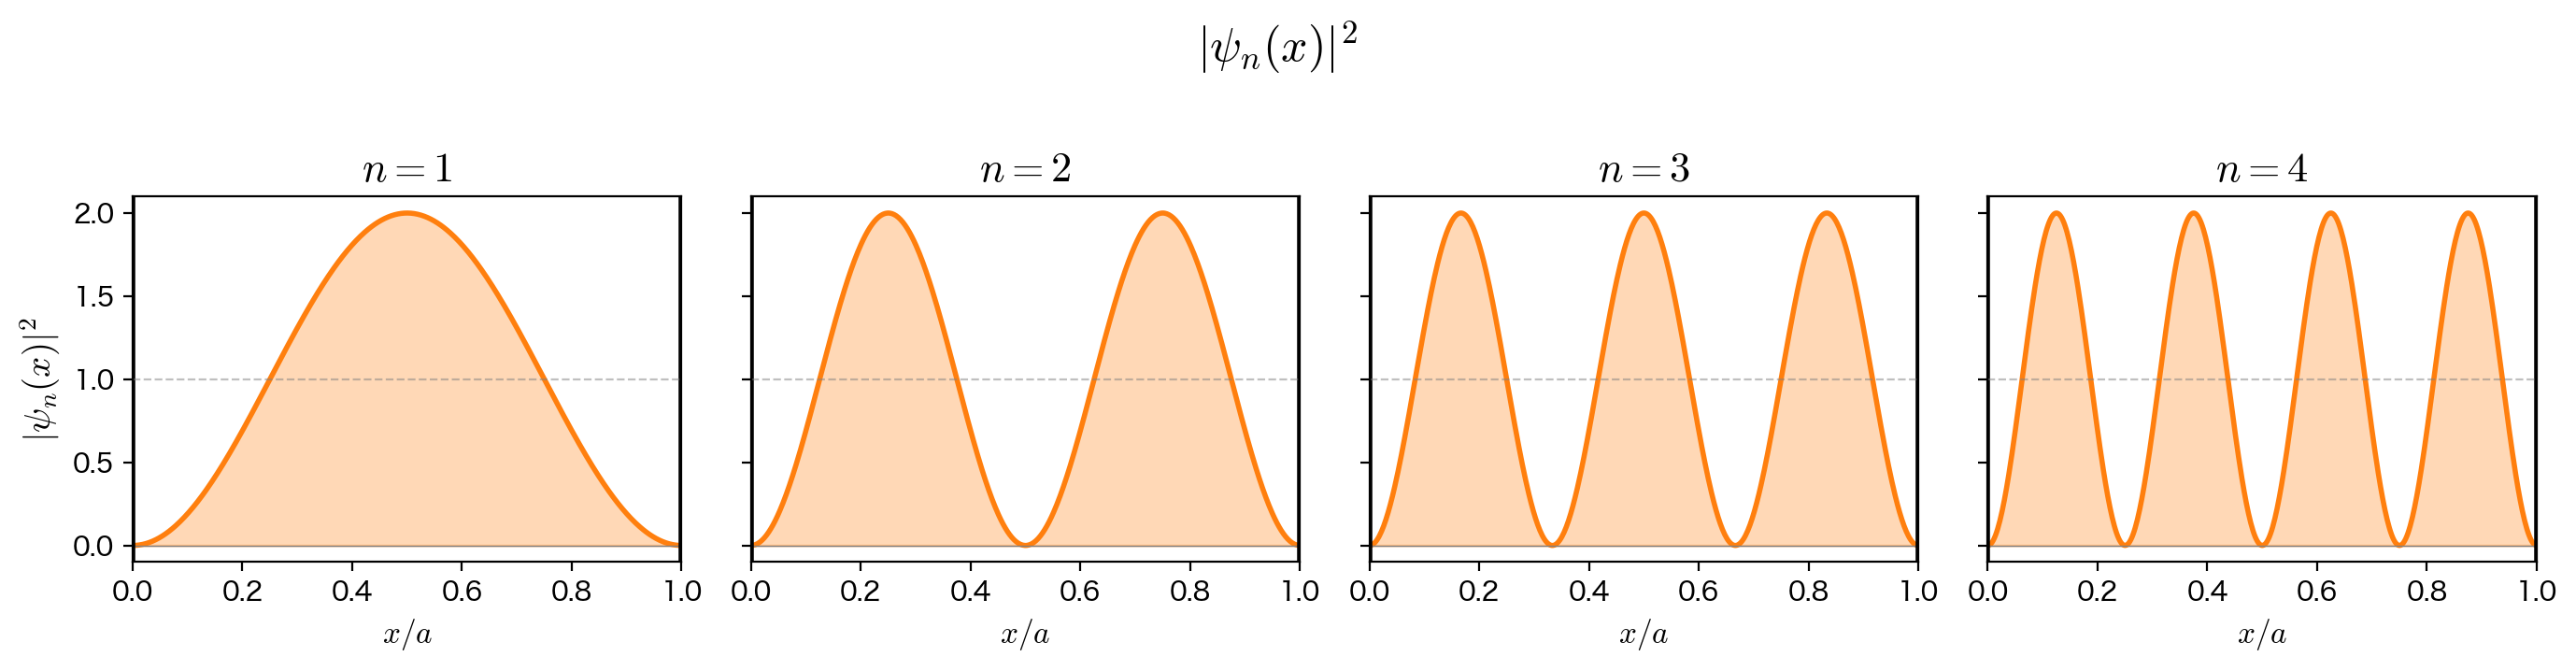
\includegraphics[width=\textwidth]{figures/probability_density.png}\\
  {\small $|\psi_n|^2$：灰破線＝古典極限（一様分布$1/a$）}
\end{column}
\end{columns}

\vspace{0.3em}
\teacher{図から読み取れること：}
\begin{itemize}
  \item $n = 1$：箱の中央に最も存在しやすい
  \item $n = 2$：中央で$|\psi|^2 = 0$（\alert{そこには絶対にいない}！）
  \item 節の数 $= n - 1$ 個
  \item $n$が大きくなると振動が激しくなる
\end{itemize}
\end{frame}

\note{
【讲解要点】\\[4pt]
\textbf{看图讲解（左图——波函数$\psi_n(x)$）：}\\
- $n=1$：半个$\sin$波，没有节点\\
- $n=2$：完整的$\sin$波，中间有1个节点\\
- $n=3$：1.5个$\sin$波，2个节点\\
- 红色圆圈标出节点位置\\
- 规律：第$n$个态有$n-1$个节点\\[4pt]
\textbf{看图讲解（右图——概率密度$|\psi_n|^2$）：}\\
- $n=1$：中间概率最大，两端为零\\
- $n=2$：中间概率为零！（反直觉——粒子"穿不过"节点）\\
- 灰色虚线是$1/a$，代表经典力学的均匀分布\\
- $n$越大，振荡越剧烈，平均后越接近经典极限\\[4pt]
\textbf{经典对应：}\\
- 经典力学中，粒子在箱子里匀速来回反弹，各处概率相等\\
- 量子力学中，$n$很大时概率密度剧烈振荡，平均值趋近$1/a$\\
- 这就是"对应原理"的体现\\[4pt]
\textbf{入试考点：}常问"$n=2$态中间概率为什么是零？"
}

% ============================================================
\begin{frame}{エネルギー準位図}

\begin{columns}[c]
\begin{column}{0.4\textwidth}
  \centering
  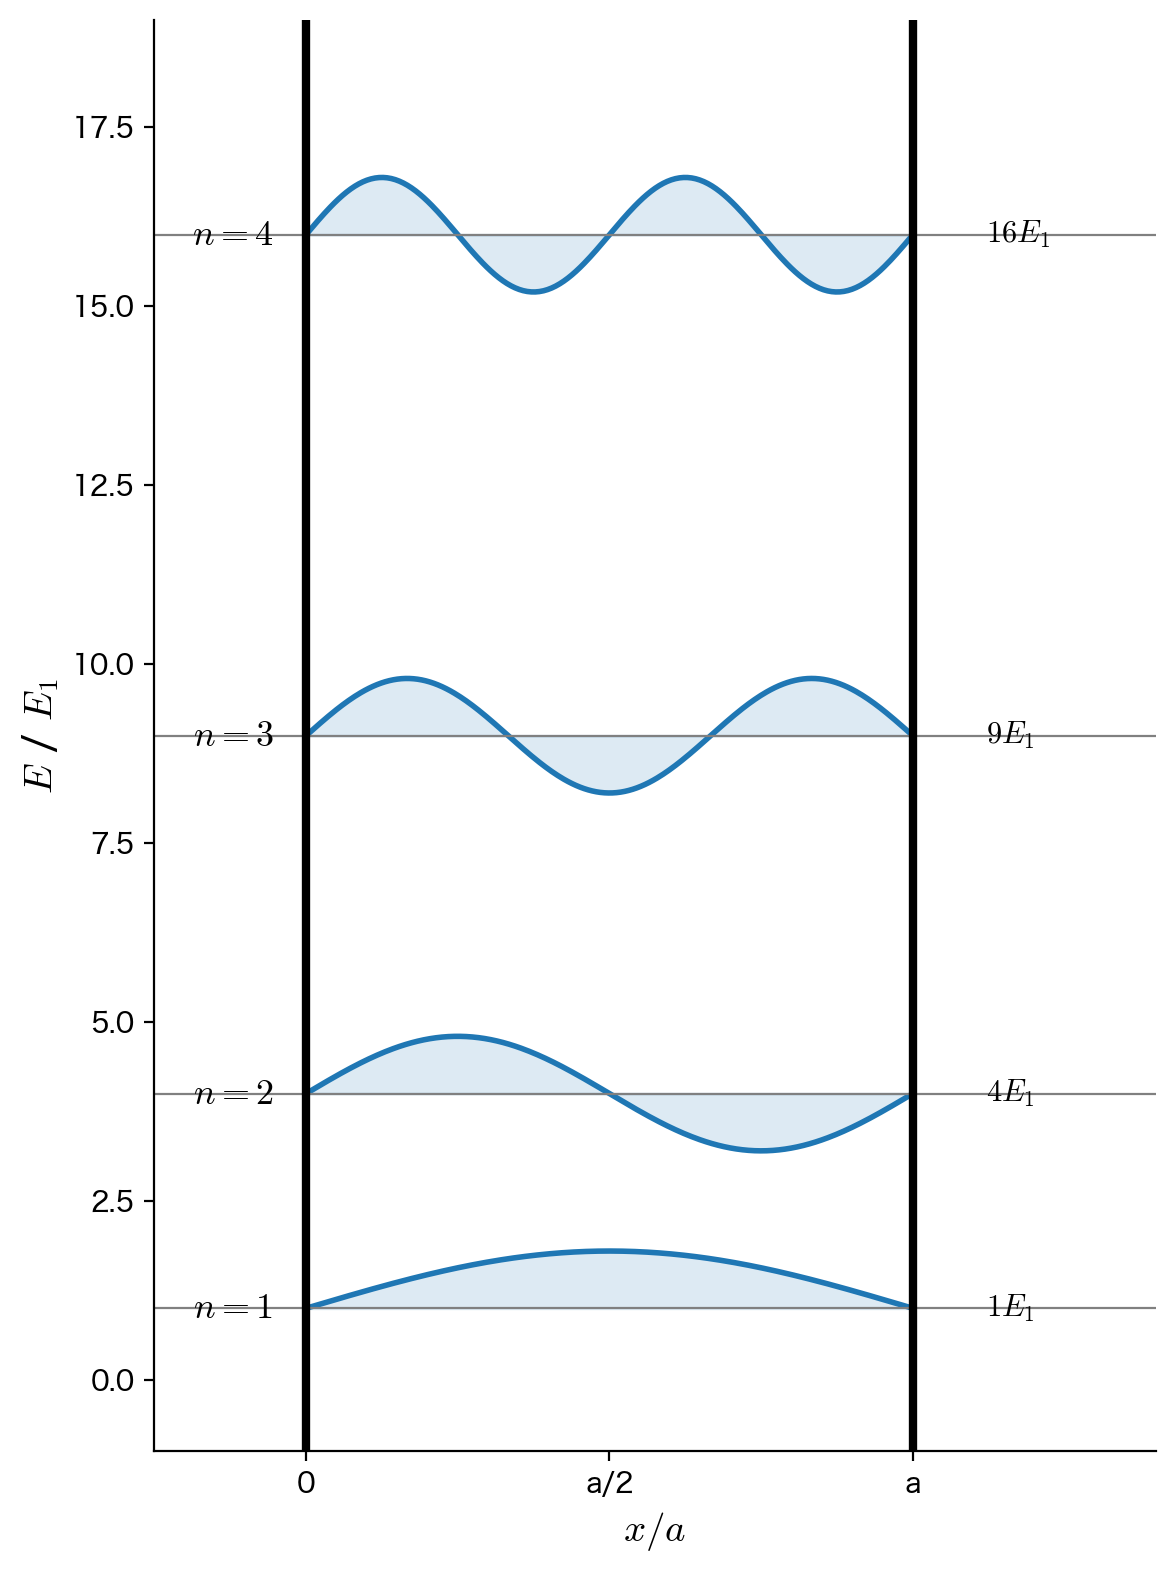
\includegraphics[width=0.95\textwidth]{figures/energy_levels_with_psi.png}
\end{column}
\begin{column}{0.6\textwidth}
  $E_n = n^2 E_1$，\quad $E_1 = h^2/(8ma^2)$

  \vspace{0.3em}
  \begin{tabular}{cccc}
    \toprule
    $n$ & $E_n/E_1$ & 節の数 & 備考 \\
    \midrule
    1 & 1 & 0 & ← \textbf{基底状態} \\
    2 & 4 & 1 & \\
    3 & 9 & 2 & \\
    4 & 16 & 3 & \\
    \bottomrule
  \end{tabular}

  \vspace{0.3em}
  \textbf{規則：}
  \begin{itemize}
    \item 節の数 $= n - 1$
    \item $\Delta E = E_{n+1} - E_n = (2n+1)E_1$\\
      → $n$が大きいほど間隔が\textbf{広がる}
  \end{itemize}
\end{column}
\end{columns}
\end{frame}

\note{
【讲解要点】\\[4pt]
\textbf{能级图的读法：}\\
- 左图：纵轴是能量，每条横线代表一个允许的能级\\
- 每个能级旁边画了对应的波函数$\psi_n$\\
- 能级间距\textbf{不均匀}，越往上越宽\\[4pt]
\textbf{数值规律（对照表格）：}\\
- $E_1 : E_2 : E_3 : E_4 = 1 : 4 : 9 : 16$（$n^2$比例）\\
- $n=1$：基态（ground state），没有节点\\
- 节点数 = $n - 1$\\[4pt]
\textbf{能级间距：}\\
- $\Delta E = E_{n+1} - E_n = [(n+1)^2 - n^2]E_1 = (2n+1)E_1$\\
- $n$越大，间距越大（与调和振子不同！调和振子是等间距）\\[4pt]
\textbf{入试常考：}\\
- 画能级图并标注波函数\\
- 计算相邻能级间距\\
- 判断节点数
}

% ============================================================
\begin{frame}{零点エネルギー}

\teacher{$n = 0$が許されないということは，\\
粒子は完全に静止できない＝エネルギーがゼロにならないということです。}

\[
  E_1 = \frac{h^2}{8ma^2} \neq 0 \qquad \text{（\textbf{零点エネルギー}）}
\]

\vspace{0.3em}
\textbf{\color{accent}なぜか？ → Heisenbergの不確定性原理で説明できます：}
\[
  \Delta x \cdot \Delta p \geq \frac{\hbar}{2}
\]

\begin{itemize}
  \item 箱に閉じ込める → 位置の不確定さ$\Delta x \leq a$
  \item すると運動量の不確定さ$\Delta p \geq \hbar/(2a)$
  \item 運動量がゼロにならない → エネルギーもゼロにならない
\end{itemize}

\vspace{0.3em}
\teacher{「閉じ込めるほど不確定性原理が効いてエネルギーが上がる」\\
これが量子力学の本質的な結論です。}

\end{frame}

\note{
【讲解要点】\\[4pt]
\textbf{零点能（zero-point energy）：}\\
- $n$最小是1，不能是0 → $E$最小是$E_1 > 0$\\
- 也就是说，粒子永远不能完全静止！这在经典力学中不可能\\[4pt]
\textbf{用海森堡不确定性原理解释（入试常考论述题）：}\\
1. 粒子被限制在长度$a$的箱子里 → 位置不确定度$\Delta x \leq a$\\
2. 不确定性原理：$\Delta x \cdot \Delta p \geq \hbar/2$\\
3. $\Delta x$有上限 → $\Delta p$有下限 → $\Delta p \geq \hbar/(2a)$\\
4. 动量不可能确切为零 → 动能不可能为零 → $E > 0$\\[4pt]
\textbf{直觉理解：}\\
- 你越想把粒子关紧（$a$越小），它就越"躁动"（$E_1$越大）\\
- 就像抓一只猫，手越紧它挣扎得越厉害\\[4pt]
\textbf{入试提示：}"用不确定性原理说明零点能不为零"是经典论述题，请务必掌握上面的三步推理。
}

% ============================================================
\begin{frame}{対応原理：古典力学との橋渡し}

\teacher{量子力学と古典力学はどう繋がるのでしょうか？}

\vspace{0.3em}
\textbf{対応原理（Bohr）：}$n \to \infty$で量子力学は古典力学に一致する。

\begin{center}
  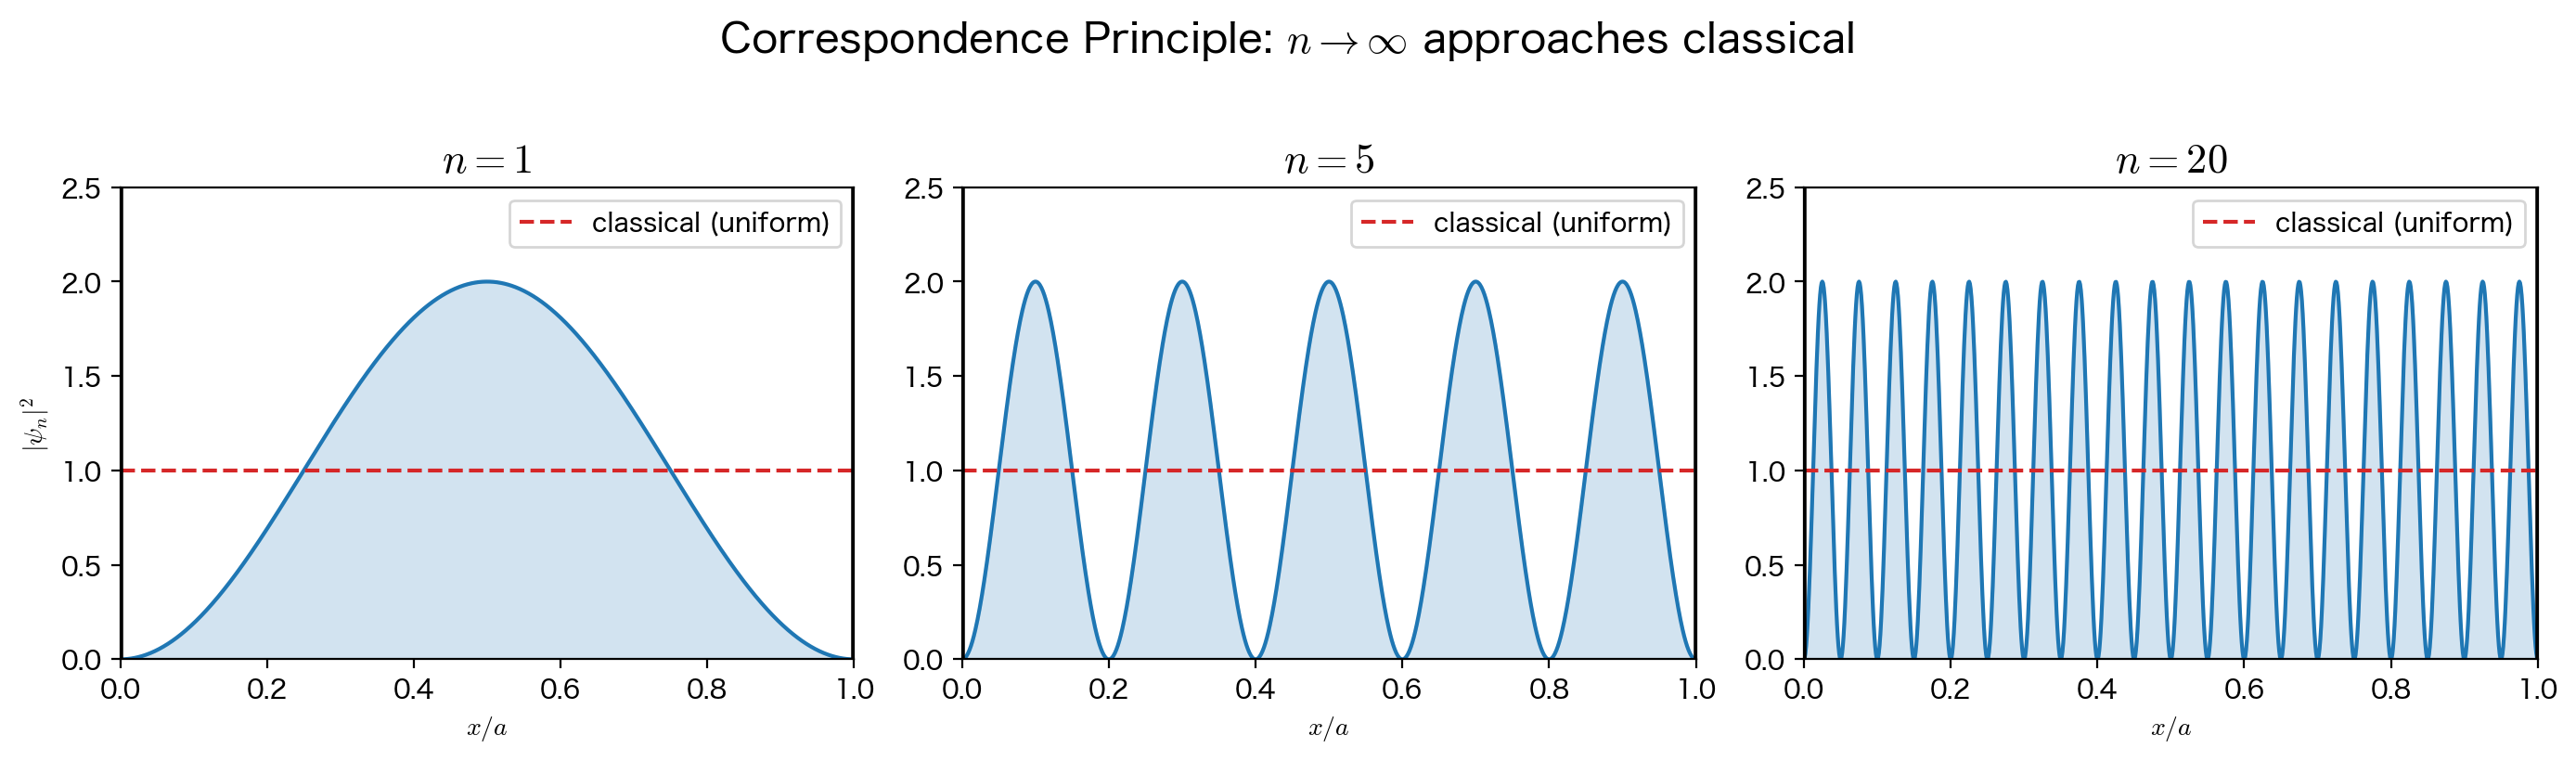
\includegraphics[width=0.65\textwidth]{figures/correspondence.png}
\end{center}

\vspace{-0.5em}
\begin{itemize}
  \item $n = 1$：中央に偏る → 古典力学と異なる
  \item $n = 20$：平均するとほぼ一様 → \textbf{古典的！}
  \item $\Delta E / E_n = (2n+1)/n^2 \to 0$（$n \to \infty$）→ 事実上連続
\end{itemize}
\end{frame}

\note{
【讲解要点】\\[4pt]
\textbf{对应原理（玻尔提出）：}\\
- 当量子数$n$趋向无穷大时，量子力学的结果趋向经典力学\\
- 这保证了量子力学和经典力学不矛盾，是一种"包含"关系\\[4pt]
\textbf{看图说话：}\\
- $n=1$：概率密度集中在中间，跟经典的均匀分布差别很大\\
- $n=20$：概率密度剧烈振荡，但平均值趋近均匀分布 → 趋近经典结果\\[4pt]
\textbf{能量也趋向连续：}\\
- 相邻能级的相对间距：$\Delta E / E_n = (2n+1)/n^2$\\
- 当$n \to \infty$：$(2n+1)/n^2 \approx 2/n \to 0$\\
- 能级间距相对于能量本身变得无穷小 → 实质上连续\\[4pt]
\textbf{总结：}量子力学是比经典力学更"基本"的理论，经典力学是量子力学在大量子数下的特殊情况。
}

% %%%%%%%%%%%%%%%%%%%%%%%%%%%%%%%%%%%%%%%%%%%%%%%%%%%%%%%%%%%%
\section{応用：共役ポリエン}
% %%%%%%%%%%%%%%%%%%%%%%%%%%%%%%%%%%%%%%%%%%%%%%%%%%%%%%%%%%%%

% ============================================================
\begin{frame}{共役ポリエンの$\pi$電子モデル}

\teacher{最後に，化学への応用を見ましょう。\\
共役ポリエンの$\pi$電子は「箱の中の粒子」で近似できます。}

\vspace{0.3em}
\textbf{モデル：}
\begin{itemize}
  \item $\pi$電子は分子骨格に沿って自由に動ける → 「箱」
  \item 箱の長さ$a \approx$（結合の数）$\times$（C--C結合長 $\approx \SI{0.14}{nm}$）
  \item Pauliの排他原理：各準位に電子は最大2個（$\uparrow\downarrow$）
\end{itemize}

\vspace{0.3em}
\textbf{用語：}
\begin{itemize}
  \item \textbf{HOMO}：電子が入っている最も高い準位
  \item \textbf{LUMO}：電子が入っていない最も低い準位
  \item 光吸収 ＝ 電子がHOMO → LUMOに遷移
\end{itemize}
\end{frame}

\note{
【讲解要点】\\[4pt]
\textbf{化学应用——共轭多烯的$\pi$电子模型：}\\
- 共轭多烯（如丁二烯CH\textsubscript{2}=CH-CH=CH\textsubscript{2}）的$\pi$电子可以在整个分子骨架上自由移动\\
- 可以近似为"箱中粒子"！箱的长度 = 共轭链长\\[4pt]
\textbf{模型设定：}\\
- 箱长$a$：大约 = 键的数目 $\times$ C-C键长（约0.14 nm）\\
- 泡利不相容原理：每个能级最多放2个电子（自旋相反$\uparrow\downarrow$）\\[4pt]
\textbf{重要术语：}\\
- HOMO（Highest Occupied Molecular Orbital）：有电子占据的最高能级\\
- LUMO（Lowest Unoccupied Molecular Orbital）：没有电子占据的最低能级\\
- 光吸收 = 电子从HOMO跃迁到LUMO\\
- 吸收光的能量 = LUMO和HOMO的能量差\\[4pt]
\textbf{过渡：}下面用丁二烯做一个具体的计算例子。
}

% ============================================================
\begin{frame}{ブタジエンの吸収波長を計算する}

\begin{columns}[c]
\begin{column}{0.6\textwidth}
\textbf{ブタジエン}（4個の$\pi$電子，$a \approx \SI{0.42}{nm}$）

$n=1$に2個，$n=2$に2個 → HOMO: $n=2$，LUMO: $n=3$

\vspace{0.3em}
HOMO→LUMO遷移（$n = 2 \to 3$）：
\[
  \Delta E = 5 \cdot \frac{h^2}{8ma^2} \approx \SI{1.7e-18}{J}
\]
\[
  \lambda = hc/\Delta E \approx \SI{117}{nm}
\]
{\small （実測$\approx \SI{217}{nm}$：モデルの限界）}
\end{column}
\begin{column}{0.4\textwidth}
  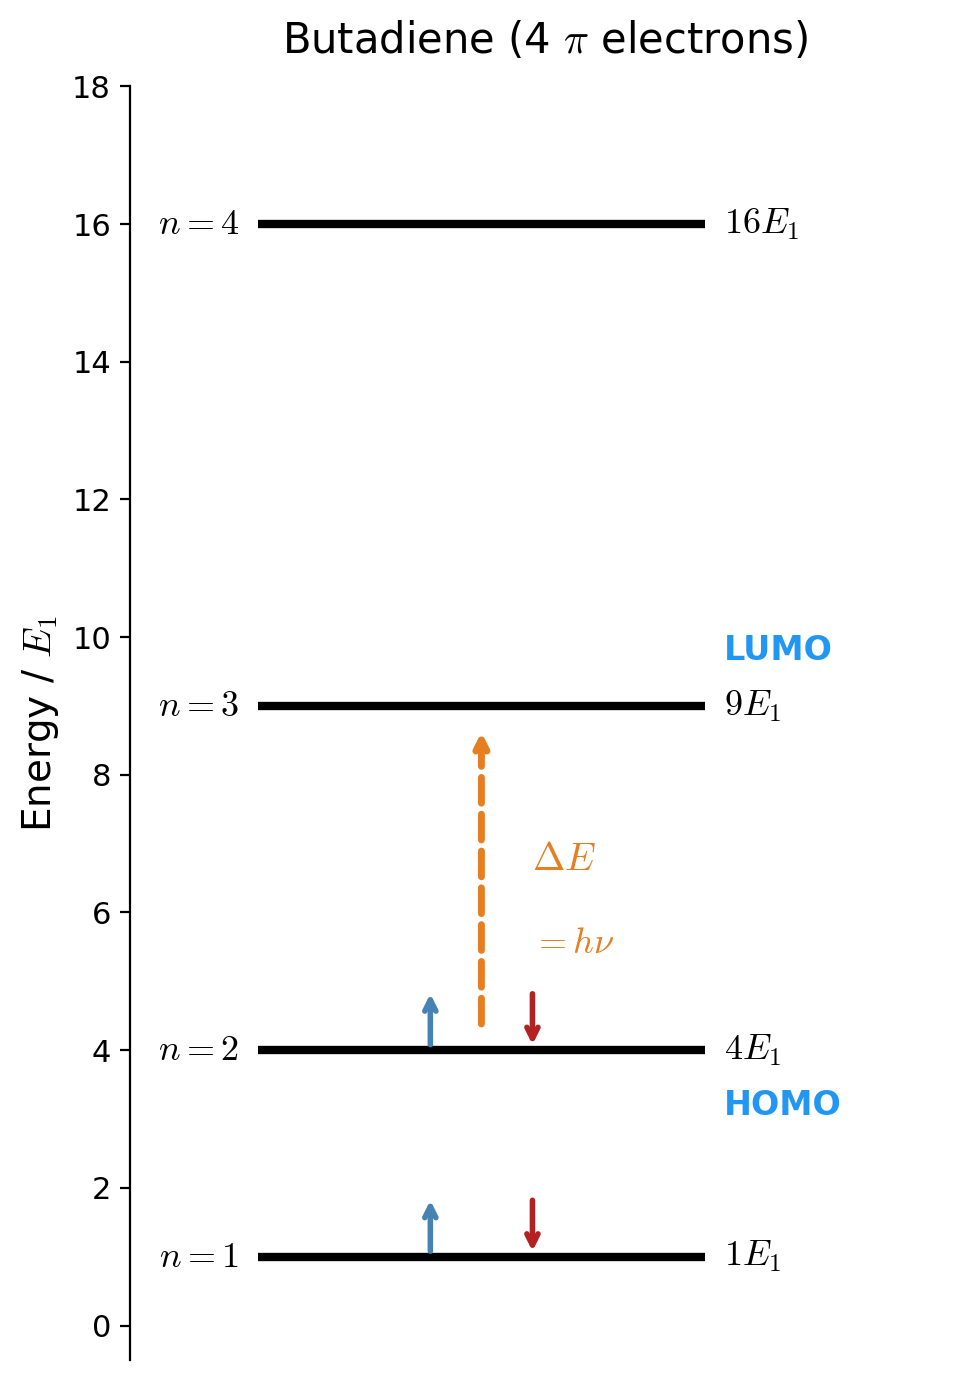
\includegraphics[width=0.85\textwidth]{figures/butadiene_levels.png}
\end{column}
\end{columns}
\end{frame}

\note{
【讲解要点】\\[4pt]
\textbf{丁二烯的具体计算：}\\
- 丁二烯有4个$\pi$电子\\
- 填入能级：$n=1$放2个，$n=2$放2个 → HOMO是$n=2$，LUMO是$n=3$\\[4pt]
\textbf{能量差计算：}\\
- $\Delta E = E_3 - E_2 = (9 - 4) \cdot E_1 = 5E_1$\\
- $E_1 = h^2/(8ma^2)$，$a \approx 0.42$ nm，$m$ = 电子质量\\
- 算出$\Delta E \approx 1.7 \times 10^{-18}$ J\\[4pt]
\textbf{波长计算：}\\
- $\lambda = hc/\Delta E \approx 117$ nm\\
- 实验值约217 nm → 模型偏差较大\\
- 原因：箱中粒子模型太简化了（忽略了电子间排斥、势能不是真正的方形势阱等）\\[4pt]
\textbf{虽然数值不精确，但定性趋势是对的：}\\
共轭链越长 → $a$越大 → $\Delta E$越小 → $\lambda$越长（红移）\\[4pt]
\textbf{入试提示：}计算HOMO→LUMO跃迁的$\Delta E$和$\lambda$是经典考题。
}

% ============================================================
\begin{frame}{共役の長さと色の関係}

\importantbox{
  共役系が長くなる → $a$が増大 → $\Delta E$が減少 → $\lambda$が\alert{赤方偏移}
}

\vspace{0.3em}
\begin{center}
\begin{tabular}{lcccc}
  \toprule
  分子 & $\pi$電子数 & HOMO & LUMO & 傾向 \\
  \midrule
  エチレン & 2 & $n=1$ & $n=2$ & 短波長（UV） \\
  ブタジエン & 4 & $n=2$ & $n=3$ & ↓ \\
  ヘキサトリエン & 6 & $n=3$ & $n=4$ & ↓ \\
  $\beta$-カロテン & 22 & $n=11$ & $n=12$ & 可視光（橙色！） \\
  \bottomrule
\end{tabular}
\end{center}

\vspace{0.3em}
\teacher{にんじんが橙色なのは，$\beta$-カロテンの共役系が長くて\\
可視光を吸収するからです。Particle in a Boxで説明できる！}

\vspace{0.3em}
\end{frame}

\note{
【讲解要点】\\[4pt]
\textbf{核心定性规律（必记！）：}\\
共轭链越长 → 箱子越大 → 能级间距越小 → 吸收光波长越长（红移）\\[4pt]
\textbf{表格逐行讲解：}\\
- 乙烯（2个$\pi$电子）：HOMO $n=1$, LUMO $n=2$，$\Delta E$大 → 吸收紫外线\\
- 丁二烯（4个）：$\Delta E$稍小\\
- 己三烯（6个）：$\Delta E$更小\\
- $\beta$-胡萝卜素（22个！）：$\Delta E$小到吸收可见光（蓝紫色光被吸收，反射橙色）\\[4pt]
\textbf{生活中的化学：}\\
- 胡萝卜是橙色的，因为$\beta$-胡萝卜素的共轭链有22个$\pi$电子\\
- 共轭链足够长，可以吸收可见光中的蓝紫色部分\\
- 互补色就是橙色！\\
- 用箱中粒子就能解释！\\[4pt]
\textbf{过渡：}到这里我们讲完了箱中粒子模型。接下来看另一个重要模型——分子振动（调和振子）。
}

% %%%%%%%%%%%%%%%%%%%%%%%%%%%%%%%%%%%%%%%%%%%%%%%%%%%%%%%%%%%%
\section{もう一つの重要な例：分子振動}
% %%%%%%%%%%%%%%%%%%%%%%%%%%%%%%%%%%%%%%%%%%%%%%%%%%%%%%%%%%%%

% ============================================================
\begin{frame}{箱の次は「ばね」：調和振動子}

\teacher{井戸型ポテンシャルの次に大事なのが，\textbf{分子の振動}です。\\
二原子分子の結合を「ばね」と見なすと，調和振動子になります。}

\vspace{0.3em}
\textbf{ポテンシャル：}
\[
  V^\text{H} = \frac{1}{2}k(R - R_e)^2 = \frac{1}{2}kx^2
\]
{\small $k$：ばね定数，$R_e$：平衡結合距離，$x = R - R_e$：変位}

\vspace{0.3em}
\textbf{時間に依存しないSchrödinger方程式：}
\[
  -\frac{\hbar^2}{2\mu}\frac{d^2\psi}{dx^2} + \frac{1}{2}kx^2\psi = E\psi
\]
{\small $\mu$：\textbf{換算質量}（reduced mass）$= m_1 m_2/(m_1 + m_2)$}

\vspace{0.3em}
\teacher{井戸型と違って$V(x)$が$x^2$に比例するので，解はもっと複雑になります。\\
でも結果はとてもシンプルです。}
\end{frame}

\note{
【讲解要点】\\[4pt]
\textbf{从"箱子"到"弹簧"：}\\
- 箱中粒子：$V$要么是0要么是$\infty$（不太现实）\\
- 调和振子：$V = \frac{1}{2}kx^2$（抛物线形），更接近真实分子\\
- 双原子分子的化学键可以看作一个"弹簧"\\[4pt]
\textbf{关键参数：}\\
- $k$：力常数（弹簧的"硬度"），单位N/m，反映键的强度\\
- $R_e$：平衡键长（弹簧自然长度）\\
- $x = R - R_e$：偏离平衡位置的位移\\
- $\mu$：约化质量 $= m_1 m_2/(m_1+m_2)$（两体问题简化为一体）\\[4pt]
\textbf{为什么用约化质量？}\\
- 两个原子都在振动，不是一个固定一个动\\
- 约化质量是把两体振动等价为一个质量为$\mu$的粒子在弹性势场中运动\\[4pt]
\textbf{过渡：}方程的解法比较复杂（涉及Hermite多项式），但结果很简洁，下一页直接给出。
}

% ============================================================
\begin{frame}{調和振動子のエネルギー準位}

\begin{columns}[c]
\begin{column}{0.45\textwidth}
  \centering
  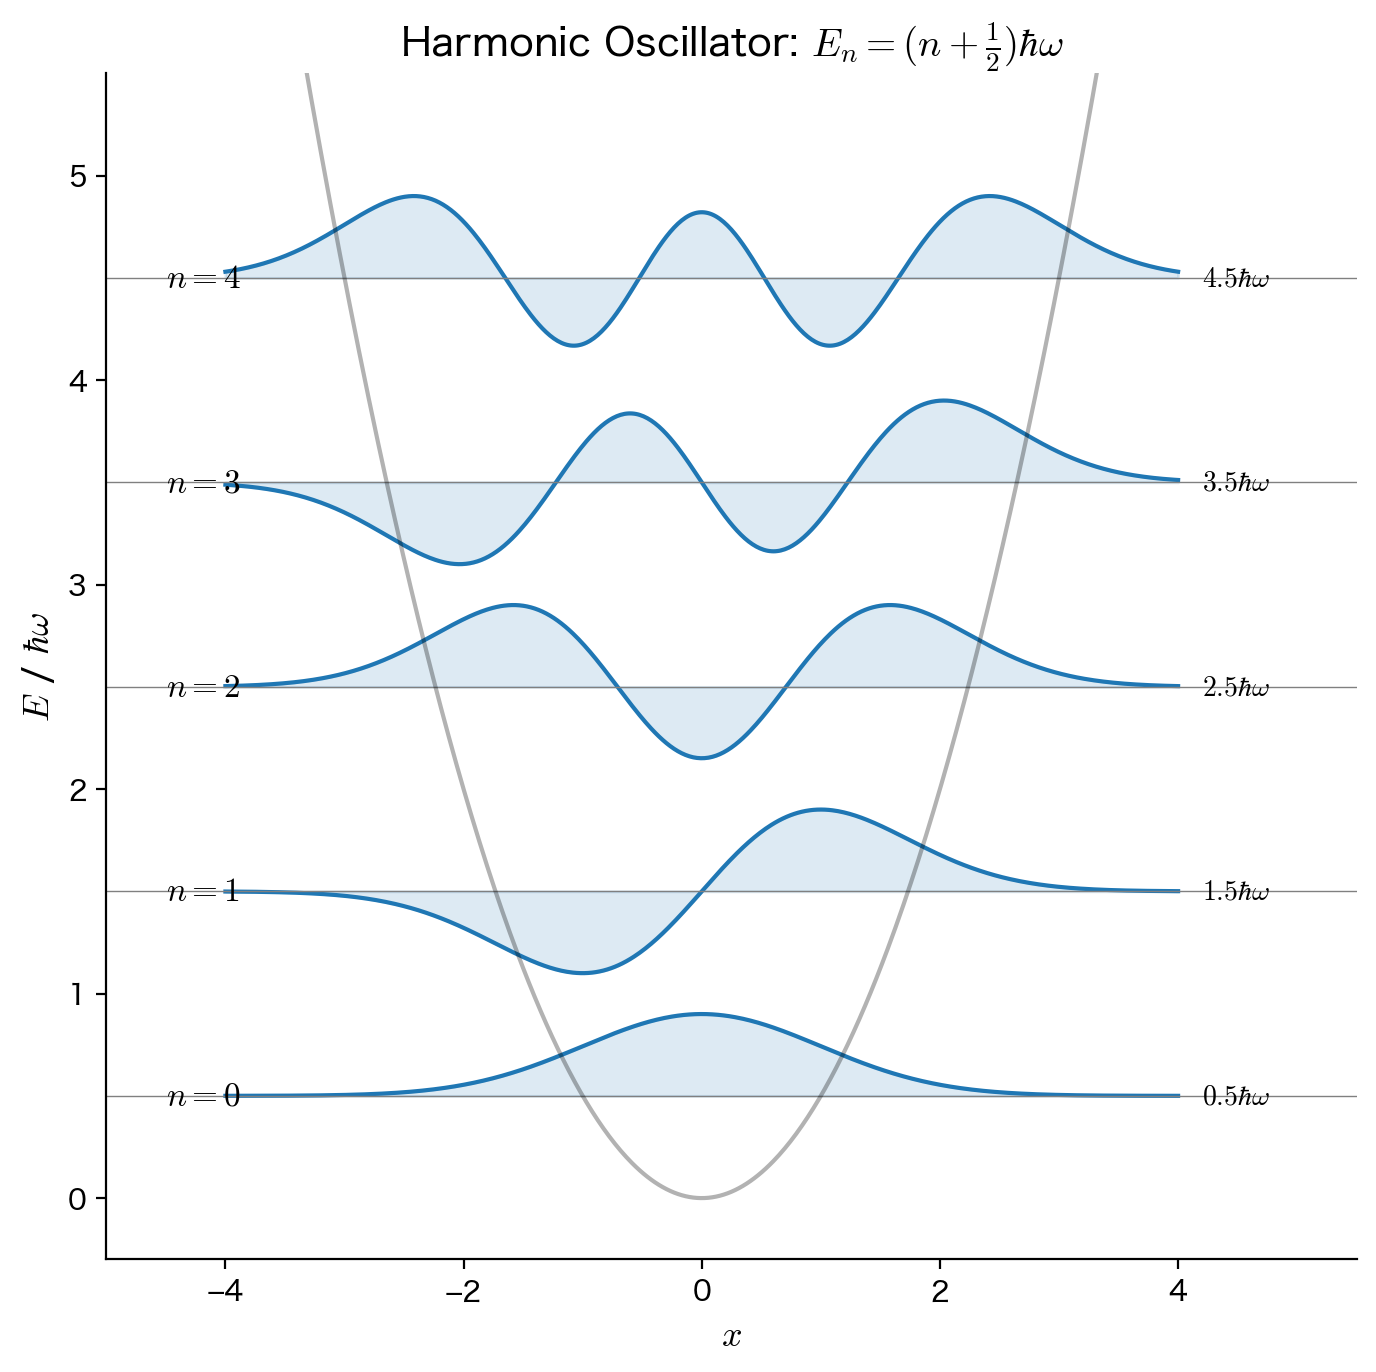
\includegraphics[width=\textwidth]{figures/harmonic_oscillator.png}
\end{column}
\begin{column}{0.55\textwidth}
\importantbox{
  \[
    E_n = \left(n + \frac{1}{2}\right)\hbar\omega, \quad n = 0, 1, 2, \ldots
  \]
  $\omega = \sqrt{k/\mu}$：角振動数
}

\vspace{0.3em}
\textbf{井戸型ポテンシャルとの比較：}

\begin{tabular}{lcc}
  \toprule
  & 井戸型 & 調和振動子 \\
  \midrule
  $E_n$ & $\propto n^2$ & $\propto n$ \\
  間隔 & 不均一 & \alert{等間隔} $\hbar\omega$ \\
  零点E & $E_1 \neq 0$ & $E_0 = \frac{1}{2}\hbar\omega \neq 0$ \\
  量子数 & $n = 1,2,3,\ldots$ & $n = 0,1,2,\ldots$ \\
  \bottomrule
\end{tabular}
\end{column}
\end{columns}

\vspace{0.3em}
\teacher{波数$\tilde{\nu}$で表すと：$E_n = (n+\frac{1}{2})hc\tilde{\nu}$。\\
赤外吸収の波数がそのまま$\tilde{\nu}$に対応します。}
\end{frame}

\note{
【讲解要点】\\[4pt]
\textbf{调和振子能级公式（必背！）：}\\
$E_n = (n + \frac{1}{2})\hbar\omega$，$n = 0, 1, 2, \ldots$\\
- $\omega = \sqrt{k/\mu}$：角频率\\
- 零点能：$E_0 = \frac{1}{2}\hbar\omega$（$n=0$时能量不为零）\\[4pt]
\textbf{与箱中粒子的对比（非常重要的区别）：}\\
1. 能级间距：箱中粒子是$\propto n^2$（不均匀），调和振子是\textbf{等间距}$\hbar\omega$\\
2. 量子数：箱中粒子从$n=1$开始，调和振子从$n=0$开始\\
3. 两者都有零点能\\[4pt]
\textbf{波数表示：}\\
- 红外光谱常用波数$\tilde{\nu}$（单位cm$^{-1}$）\\
- $E_n = (n+\frac{1}{2})hc\tilde{\nu}$\\
- 基本吸收对应$n=0 \to 1$，吸收能量恰好是$hc\tilde{\nu}$\\
- 所以红外光谱中的吸收峰位置就直接给出了$\tilde{\nu}$\\[4pt]
\textbf{看图：}左图是抛物线势阱中的等间距能级，波函数画在每个能级上。
}

% ============================================================
\begin{frame}{赤外吸収の選択律}

\teacher{調和振動子のエネルギー間隔は等間隔$\hbar\omega$なので，\\
赤外光を吸収するときの条件はシンプルです。}

\vspace{0.3em}
\textbf{選択律（selection rule）：}
\importantbox{
  $\Delta n = \pm 1$ \quad （基本振動のみ許される）
}

\textbf{赤外吸収のもう一つの条件：}

振動に伴い\textbf{双極子モーメントが変化}すること

\teacher{対称分子（H$_2$, N$_2$）は振動しても双極子が変わらない → 赤外不活性}
\end{frame}

\note{
【讲解要点】\\[4pt]
\textbf{选择定则（调和振子）：}\\
- 只允许$\Delta n = \pm 1$的跃迁（吸收或发射一个量子）\\
- 也就是说，$n=0 \to 1$可以，$n=0 \to 2$不行\\
- 这是调和振子模型的结论，真实分子（非谐性）可以有$\Delta n = 2, 3, \ldots$（倍频）\\[4pt]
\textbf{红外活性的条件：}\\
- 光吸收涉及电磁场与分子的相互作用\\
- 只有振动引起\textbf{偶极矩变化}时，才能与电磁波耦合\\[4pt]
\textbf{举例：}\\
- HCl：振动时H和Cl之间的电荷分布变化 → 偶极矩变化 → 红外活性\\
- H$_2$、N$_2$：对称分子，振动时偶极矩始终为零 → 红外不活性\\
- CO$_2$：对称伸缩模式不活性，但反对称伸缩模式活性\\[4pt]
\textbf{入试考点：}判断哪些分子/振动模式是红外活性的。
}

% ============================================================
\begin{frame}{赤外活性と基準振動モード}

\begin{tabular}{lcl}
  \toprule
  分子 & 赤外活性？ & 理由 \\
  \midrule
  HCl, CO, H$_2$O & ○ & 双極子モーメントが変化 \\
  H$_2$, N$_2$, O$_2$ & × & 対称 → 双極子変化なし \\
  CO$_2$（逆対称伸縮） & ○ & 非対称モードで双極子変化 \\
  \bottomrule
\end{tabular}

\vspace{0.6em}
\textbf{基準振動モード数：}
\begin{itemize}
  \item 非直線分子：$3N - 6$
  \item 直線分子：$3N - 5$
\end{itemize}

{\small 例：CO$_2$（直線，$N=3$）→ $3\times3 - 5 = 4$モード}
\end{frame}

\note{
【讲解要点】\\[4pt]
\textbf{红外活性总结表：}\\
- HCl、CO、H$_2$O：有永久偶极矩或振动时偶极矩变化 → 红外活性\\
- H$_2$、N$_2$、O$_2$：同核双原子，完全对称 → 振动不改变偶极矩 → 不活性\\
- CO$_2$：虽然是对称的，但反对称伸缩模式会产生偶极矩变化 → 该模式活性\\[4pt]
\textbf{基准振动模式数（必记公式）：}\\
- 非线性分子：$3N - 6$（$N$是原子数）\\
- 线性分子：$3N - 5$\\
- 为什么？$3N$个自由度，减去3个平移+3个（或2个）转动\\[4pt]
\textbf{CO$_2$的例子：}\\
- 3个原子，线性 → $3 \times 3 - 5 = 4$个振动模式\\
- 对称伸缩（1个）、反对称伸缩（1个）、弯曲振动（2个，互相垂直但简并）\\[4pt]
\textbf{入试考点：}给定分子，求振动模式数；判断哪些模式是红外活性的。
}

% ============================================================
\begin{frame}{換算質量と振動波数の計算}

\teacher{入試では，具体的な分子の赤外吸収波数を計算させる問題がよく出ます。}

\vspace{0.3em}
\textbf{換算質量：}
\[
  \mu = \frac{m_1 m_2}{m_1 + m_2}
\]

\textbf{振動波数：}
\[
  \tilde{\nu} = \frac{1}{2\pi c}\sqrt{\frac{k}{\mu}}
\]

\vspace{0.3em}
\textbf{計算例：}$^{12}$C$^{16}$O（$k = \SI{1855}{N.m^{-1}}$）
\begin{align}
  \mu &= \frac{12 \times 16}{12 + 16} \times \frac{1}{\SI{6.02e23}{}} = \SI{1.14e-26}{kg} \\[4pt]
  \tilde{\nu} &= \frac{1}{2\pi \times \SI{3.00e8}{}}\sqrt{\frac{1855}{\SI{1.14e-26}{}}}
  \approx \SI{2150}{cm^{-1}}
\end{align}
\end{frame}

\note{
【讲解要点】\\[4pt]
\textbf{计算步骤（入试必练）：}\\[4pt]
\textbf{步骤1：求约化质量$\mu$}\\
- $\mu = \frac{m_1 m_2}{m_1 + m_2}$\\
- 注意：原子质量要用kg！\\
- 先用原子量（g/mol）计算 $\frac{M_1 M_2}{M_1 + M_2}$，再除以阿伏伽德罗常数$N_A$，再乘以$10^{-3}$转换\\[4pt]
\textbf{步骤2：求振动波数$\tilde{\nu}$}\\
- $\tilde{\nu} = \frac{1}{2\pi c}\sqrt{k/\mu}$\\
- $c$用cm/s（$3.00 \times 10^{10}$ cm/s），这样$\tilde{\nu}$直接得到cm$^{-1}$\\
- 或者$c$用m/s，$\tilde{\nu}$先得m$^{-1}$，再除100得cm$^{-1}$\\[4pt]
\textbf{CO的计算例：}\\
- $\mu = 12 \times 16 / (12 + 16) / N_A = 1.14 \times 10^{-26}$ kg\\
- $\tilde{\nu} = \frac{1}{2\pi \times 3.00 \times 10^{10}} \sqrt{1855 / 1.14 \times 10^{-26}} \approx 2150$ cm$^{-1}$\\[4pt]
\textbf{单位陷阱：}入试中单位换算是最容易丢分的地方，一定要仔细！
}

% ============================================================
\begin{frame}{実在分子：Morseポテンシャル}

\teacher{実際の分子は大きく伸ばすと解離する → 非対称ポテンシャル。}

\begin{columns}[c]
\begin{column}{0.45\textwidth}
  \centering
  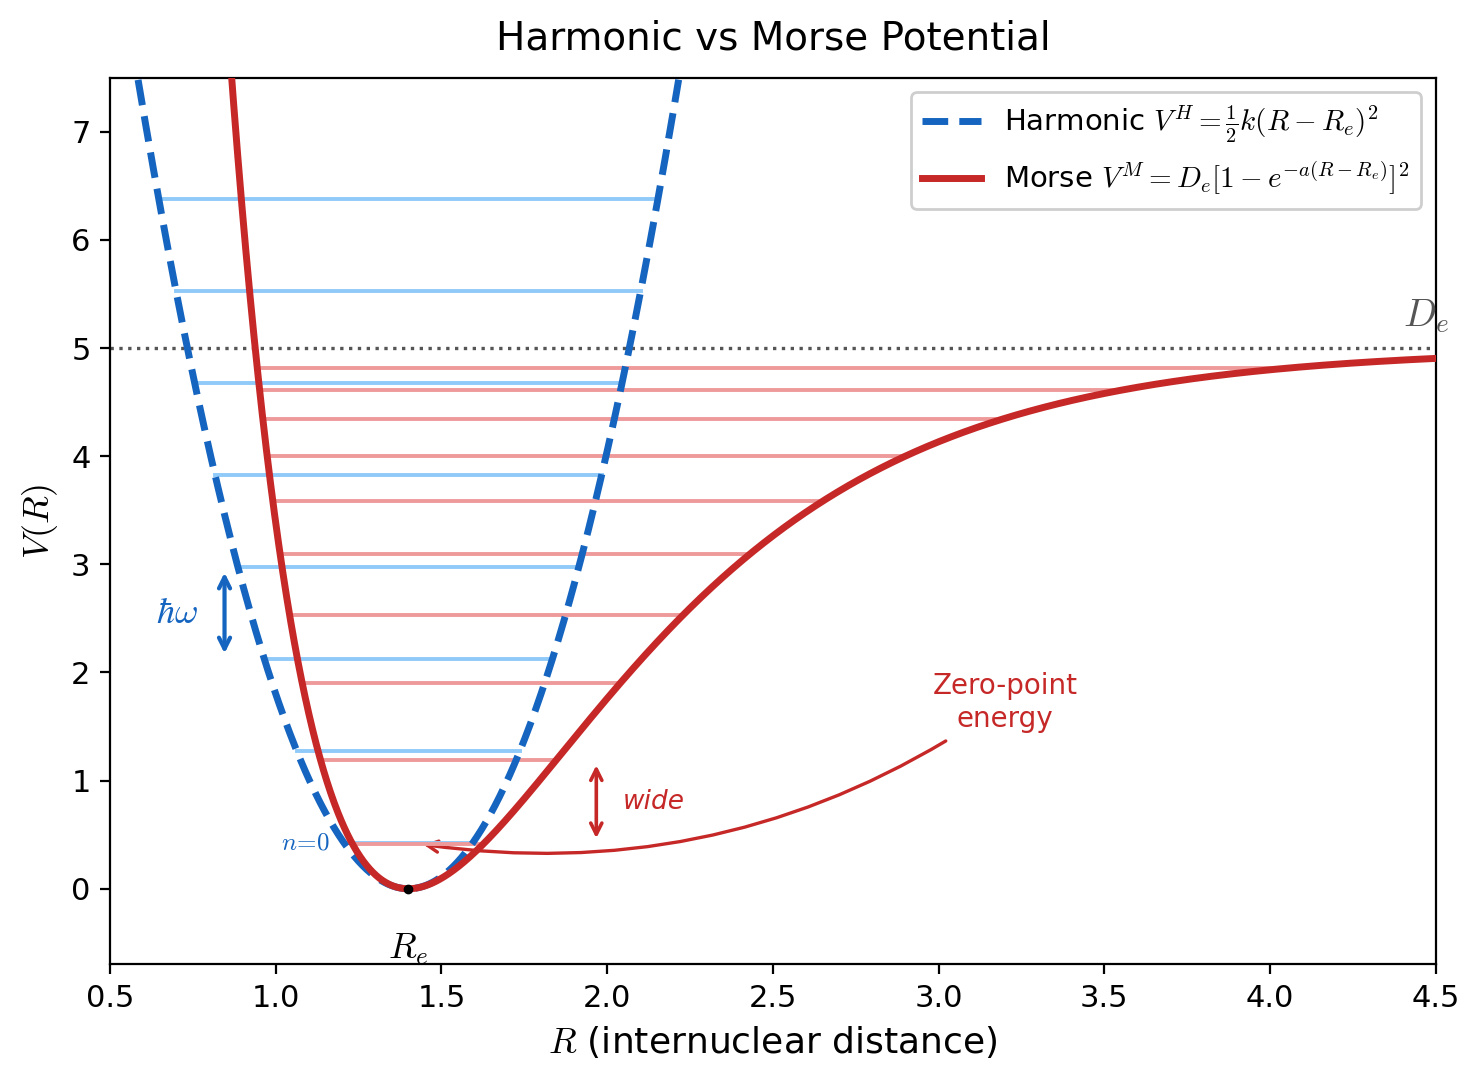
\includegraphics[width=0.95\textwidth]{figures/morse_vs_harmonic.png}
\end{column}
\begin{column}{0.55\textwidth}
$V^\text{M} = D_e[1 - e^{-a(R-R_e)}]^2$\quad{\small ($D_e$：解離エネルギー)}

\vspace{0.2em}
$E_n^\text{M} = E_n^\text{H} - (n+\tfrac{1}{2})^2 \dfrac{hc\tilde{\nu}^2}{4D_e}$

\vspace{0.3em}
\textbf{調和振動子との違い：}
\begin{itemize}
  \item 間隔が$n$とともに\alert{狭くなる}
  \item 有限個の束縛状態のみ
  \item 倍音（$\Delta n = 2,3,\ldots$）が許される
\end{itemize}
\end{column}
\end{columns}
\end{frame}

\note{
【讲解要点】\\[4pt]
\textbf{为什么需要Morse势？}\\
- 调和振子（抛物线）在平衡位置附近是好的近似\\
- 但真实分子如果被拉得很长，化学键会断裂（解离）\\
- 调和势$V \to \infty$当$x \to \infty$，不可能解离 → 不真实\\
- Morse势：$V \to D_e$当$R \to \infty$，有解离极限 → 更真实\\[4pt]
\textbf{Morse势的能级：}\\
- $E_n^M = (n+\frac{1}{2})\hbar\omega - (n+\frac{1}{2})^2 \frac{hc\tilde{\nu}^2}{4D_e}$\\
- 第二项是修正项（非谐性修正），总是负的\\
- 结果：能级间距随$n$增大而\textbf{减小}（越高越密）\\[4pt]
\textbf{三个与调和振子的关键区别（入试常考）：}\\
1. 能级间距不等，$n$越大越小\\
2. 束缚态数目有限（不能无限激发）\\
3. 倍频跃迁（$\Delta n = 2, 3, \ldots$）被允许（选择定则放宽）\\[4pt]
\textbf{看图：}红色是Morse势（不对称），蓝色虚线是调和势（对称抛物线）。
}

% %%%%%%%%%%%%%%%%%%%%%%%%%%%%%%%%%%%%%%%%%%%%%%%%%%%%%%%%%%%%
\section{黒体放射の定量的取り扱い}
% %%%%%%%%%%%%%%%%%%%%%%%%%%%%%%%%%%%%%%%%%%%%%%%%%%%%%%%%%%%%

% ============================================================
\begin{frame}{Planck分布の極限}

\teacher{黒体放射を定量的に掘り下げましょう。入試では極限の導出が頻出です。}

\begin{columns}[c]
\begin{column}{0.45\textwidth}
  \centering
  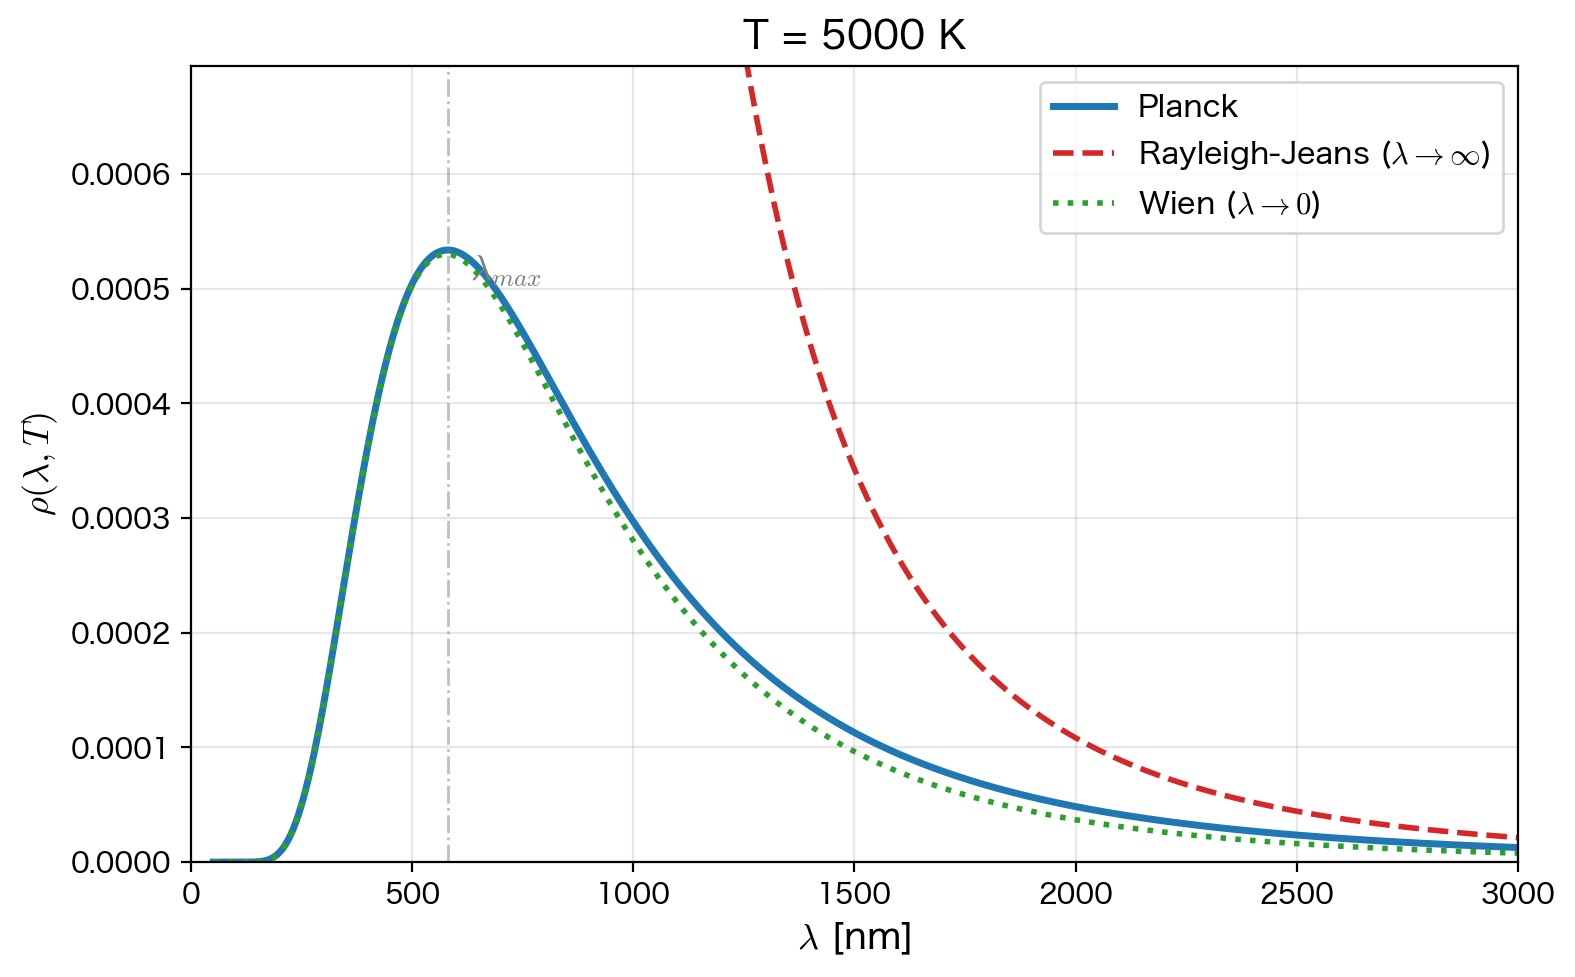
\includegraphics[width=0.95\textwidth]{figures/planck_with_limits.png}
\end{column}
\begin{column}{0.55\textwidth}
$\displaystyle\rho = \frac{8\pi hc}{\lambda^5}\frac{1}{e^{hc/\lambda k_\text{B}T} - 1}$

\vspace{0.3em}
\textbf{短波長}（$\lambda \to 0$）：$\rho \to 0$（Wien分布）

\vspace{0.2em}
\textbf{長波長}（$\lambda \to \infty$）：$e^x \approx 1+x$より
\[
  \rho \approx \frac{8\pi k_\text{B}T}{\lambda^4} \quad \text{（Rayleigh-Jeans）}
\]
\end{column}
\end{columns}
\end{frame}

\note{
【讲解要点】\\[4pt]
\textbf{普朗克分布公式（完整形式）：}\\
$\rho(\lambda,T) = \frac{8\pi hc}{\lambda^5} \cdot \frac{1}{e^{hc/(\lambda k_B T)} - 1}$\\[4pt]
\textbf{两个极限（入试常考推导）：}\\[4pt]
\textbf{1. 短波长极限（$\lambda \to 0$）→ Wien分布：}\\
- $hc/(\lambda k_B T) \to \infty$ → $e^{hc/\lambda k_B T} \gg 1$\\
- 分母中的$-1$可忽略 → $\rho \approx \frac{8\pi hc}{\lambda^5} e^{-hc/\lambda k_B T}$\\
- 指数衰减，$\rho \to 0$（解决了紫外灾难！）\\[4pt]
\textbf{2. 长波长极限（$\lambda \to \infty$）→ Rayleigh-Jeans分布：}\\
- $hc/(\lambda k_B T) \to 0$，用Taylor展开 $e^x \approx 1+x$\\
- 分母 $\approx 1 + hc/(\lambda k_B T) - 1 = hc/(\lambda k_B T)$\\
- $\rho \approx \frac{8\pi hc}{\lambda^5} \cdot \frac{\lambda k_B T}{hc} = \frac{8\pi k_B T}{\lambda^4}$\\
- 这就是经典的Rayleigh-Jeans公式！\\[4pt]
\textbf{结论：}普朗克公式在两个极限下分别回归Wien和Rayleigh-Jeans，是统一的理论。
}

% ============================================================
\begin{frame}[shrink=5]{Wien の法則とStefan-Boltzmann の法則}

\textbf{① Wienの変位則：}$\rho$が最大となる波長$\lambda_\text{max}$
\[
  \frac{d\rho}{d\lambda}\bigg|_{\lambda=\lambda_\text{max}} = 0
  \quad \Longrightarrow \quad
  \lambda_\text{max}T = \text{const}
\]

\teacher{$T$が高いほど$\lambda_\text{max}$は短波長に移動する。\\
太陽（$\sim\SI{5800}{K}$）の放射ピークが可視光域にあるのはこのため。}

\vspace{0.3em}
\textbf{② Stefan-Boltzmannの法則：}全放射エネルギー密度$U$
\[
  U = \int_0^\infty \rho(\lambda,T)\,d\lambda \propto T^4
\]

導出のポイント：$x = hc/(\lambda k_\text{B}T)$と置換し，
$\displaystyle\int_0^\infty \frac{x^3}{e^x - 1}dx = \frac{\pi^4}{15}$を使う。

\importantbox{
  $U = \dfrac{8\pi^5 k_\text{B}^4}{15h^3c^3}\,T^4 \propto T^4$
}
\end{frame}

\note{
【讲解要点】\\[4pt]
\textbf{① Wien位移定律：}\\
- 对$\rho(\lambda)$求导令其为零，找辐射峰值对应的波长$\lambda_{\max}$\\
- 结果：$\lambda_{\max} T = $ 常数（约2898 $\mu$m·K）\\
- 物理含义：温度越高，辐射峰越偏向短波长\\
- 例子：太阳表面$\sim$5800K → $\lambda_{\max} \approx 500$ nm → 可见光！\\
- 铁加热到红色（$\sim$1000K） → 再加热变白色（$\sim$5000K）\\[4pt]
\textbf{② Stefan-Boltzmann定律：}\\
- 把$\rho$对所有波长积分，得到总辐射能量密度$U$\\
- 令$x = hc/(\lambda k_B T)$进行换元\\
- 利用定积分$\int_0^\infty x^3/(e^x-1)dx = \pi^4/15$\\
- 最终：$U \propto T^4$\\
- 物理含义：辐射总能量与温度的四次方成正比\\[4pt]
\textbf{入试考点：}\\
- 推导Wien位移定律（对$\rho$求导）\\
- 推导Stefan-Boltzmann定律（换元积分）\\
- 用Wien定律计算$\lambda_{\max}$\\
这三个是高频考点，建议完整练习推导过程。
}

% %%%%%%%%%%%%%%%%%%%%%%%%%%%%%%%%%%%%%%%%%%%%%%%%%%%%%%%%%%%%
\section{まとめ}
% %%%%%%%%%%%%%%%%%%%%%%%%%%%%%%%%%%%%%%%%%%%%%%%%%%%%%%%%%%%%

% ============================================================
\begin{frame}[shrink=5]{全体のまとめ}

\begin{enumerate}
  \item \textbf{量子論の誕生}\\
    Planck → Einstein → de Broglie → Schrödinger

  \item \textbf{井戸型ポテンシャル}\\
    $\psi_n = \sqrt{2/a}\sin(n\pi x/a)$，\;$E_n = n^2 h^2/(8ma^2)$

  \item \textbf{物理的意味}\\
    $|\psi|^2$＝確率密度，零点エネルギー，対応原理

  \item \textbf{調和振動子}\\
    $E_n = (n+\frac{1}{2})\hbar\omega$，赤外吸収，Morseポテンシャル

  \item \textbf{黒体放射の定量}\\
    Planck分布の極限，Wien則，Stefan-Boltzmann則
\end{enumerate}
\end{frame}

\note{
【总结讲解】\\[4pt]
\textbf{五大板块回顾：}\\[4pt]
\textbf{1. 量子论的诞生：}从经典力学的失败到量子力学的建立\\
普朗克（能量量子化）→ 爱因斯坦（光子）→ 德布罗意（物质波）→ 薛定谔（波动方程）\\[4pt]
\textbf{2. 箱中粒子：}最重要的基本模型\\
波函数$\psi_n = \sqrt{2/a}\sin(n\pi x/a)$，能量$E_n = n^2 h^2/(8ma^2)$\\[4pt]
\textbf{3. 物理解释：}波函数的概率诠释，零点能，对应原理\\[4pt]
\textbf{4. 调和振子：}分子振动模型\\
$E_n = (n+1/2)\hbar\omega$，红外光谱，Morse势的修正\\[4pt]
\textbf{5. 黑体辐射定量：}普朗克分布的极限，Wien定律，Stefan-Boltzmann定律\\[4pt]
\textbf{鼓励：}这些内容看起来多，但核心其实就是"给一个$V(x)$，解薛定谔方程"这一件事。掌握了解题套路（变量分离→边界条件→归一化），就能应对入试中的大部分量子化学题目！
}

% ============================================================
\begin{frame}[shrink=5]{入試対策チェックリスト}

\begin{block}{これができれば合格ラインです：}
  {\small
  \begin{tabular}{cl}
    $\square$ & 変数分離 → 境界条件 → 規格化（半角公式）の再現 \\
    $\square$ & 零点エネルギーを不確定性原理で説明 \\
    $\square$ & 共役ポリエンの吸収波長$\lambda$の計算 \\
    $\square$ & 調和振動子の$E_n$，換算質量，振動波数 \\
    $\square$ & Morse vs 調和振動子の違いを図示 \\
    $\square$ & Planck分布の長波長/短波長極限の導出 \\
    $\square$ & Wien則・Stefan-Boltzmann則の導出 \\
  \end{tabular}
  }
\end{block}
\end{frame}

\note{
【入试备考清单讲解】\\[4pt]
\textbf{逐项检查（让听众自我评估）：}\\[4pt]
$\square$ \textbf{变量分离→边界条件→归一化}：这是最基础的，必须能从头到尾完整写出来。半角公式$\sin^2\theta = (1-\cos2\theta)/2$一定要记住。\\[4pt]
$\square$ \textbf{零点能与不确定性原理}：三步论证（位置确定→动量不确定→能量不为零），论述题常考。\\[4pt]
$\square$ \textbf{共轭多烯吸收波长}：确定HOMO/LUMO → 计算$\Delta E$ → 求$\lambda$。\\[4pt]
$\square$ \textbf{调和振子}：$E_n$公式、约化质量计算、振动波数计算。\\[4pt]
$\square$ \textbf{Morse vs 调和振子}：画图对比，说出三个区别。\\[4pt]
$\square$ \textbf{Planck分布极限}：Taylor展开$e^x \approx 1+x$要熟练。\\[4pt]
$\square$ \textbf{Wien和SB定律}：推导过程要练习。\\[4pt]
\textbf{最后鼓励：}如果这些都能做到，量子化学部分就没问题了！加油！
}

% ============================================================
\begin{frame}[standout]
  頑張れ！
\end{frame}

\note{
加油！相信自己，量子化学没有想象中那么难。掌握了今天的内容，入试的量子部分就稳了！祝大家考试顺利！
}

\end{document}
